\documentclass{beamer}

\usepackage[french]{babel}
\usepackage[utf8]{inputenc}
\usepackage[T1]{fontenc}
\usepackage{lmodern}
\usepackage{amsmath,amssymb,amsthm}
\usepackage{graphicx}
\usepackage{enumitem}
\usepackage{hyperref}
\usepackage{bookmark}
\usepackage{geometry}
\usepackage{tikz}
\usetikzlibrary{positioning,chains,fit,shapes,calc}
\usepackage[most]{tcolorbox}
\usepackage[dvipsnames]{xcolor}
\usepackage{animate}

\usetheme{Boadilla}
\title{TIPE : Simulation d'écoulement de fluides autour de structures solides}
\author{COADIC Alban   (n° 50170)}
\date{\today}

% T.O.D.O. block definition
\newcommand{\mytodo}[1]{
    \colorbox{green!20}{\textbf{\textcolor{green!50!black}{TODO\@: #1}}}
}

\begin{document}

\begin{frame}
    \titlepage{}
\end{frame}

\begin{frame}
    \frametitle{Plan de la présentation}
    · Equations de Navier - Stokes et implémentation\\
    · Optimisation \\
    · Capacités du solveur et vortex\\
    · Protection des batiments\\
    · Problèmes rencontrés et améliorations\\
\end{frame}

\begin{frame}{}
    \begin{center}
    \textbf{Équation de Navier-Stokes (fluide incompressible)}
\end{center}

\vspace{-0.2cm}
\[
\left\{
\begin{array}{l}
    \displaystyle \frac{\partial \mathbf{u}}{\partial t} = -\mathbf{u} \cdot \nabla \mathbf{u} + \mathbf{g} + \nu \Delta \mathbf{u} - \frac{1}{\rho} \nabla p \\[2ex]
    \nabla \cdot \mathbf{u} = 0
\end{array}
\right.
\]
\end{frame}

\begin{frame}{}
\vspace{-1.5cm}

\begin{center}
    \textbf{Équation de Navier-Stokes (fluide incompressible)}
\end{center}

\vspace{-0.2cm}
\[
\left\{
\begin{array}{l}
    \displaystyle 
    \frac{\partial \mathbf{u}}{\partial t} = 
    \textcolor{red}{-\mathbf{u} \cdot \nabla \mathbf{u}} 
    + \textcolor{ForestGreen}{\mathbf{g}} 
    + \textcolor{blue}{\nu \Delta \mathbf{u}} 
    - \textcolor{orange}{\frac{1}{\rho} \nabla p} \\[2ex]
    \textcolor{violet}{\nabla \cdot \mathbf{u} = 0}
\end{array}
\right.
\]

\vspace{0.1cm}

\begin{itemize}
    \item \small \textbf{\textcolor{Black}{Accélération}} ($\frac{\partial \mathbf{u}}{\partial t} $)=
    \textbf{\textcolor{red}{Advection}} (\textcolor{red}{$-\mathbf{u} \cdot \nabla \mathbf{u}$}) 
    $+$ \textbf{\textcolor{ForestGreen}{Forces externes}} (\textcolor{ForestGreen}{$\mathbf{g}$}) 
    $+$ \textbf{\textcolor{blue}{Viscosité}} (\textcolor{blue}{$\nu \Delta \mathbf{u}$}) 
    $-$ \textbf{\textcolor{orange}{Pression}} (\textcolor{orange}{$\frac{1}{\rho} \nabla p$})
    \item \textbf{\textcolor{violet}{Incompressibilité}} (\textcolor{violet}{$\nabla \cdot \mathbf{u} = 0$}): pas d'ajout ou de retrait de fluide
\end{itemize}

\end{frame}

\begin{frame}{Choix de l'implémentation}
\begin{columns}
    \begin{column}{0.48\textwidth}
        \begin{figure}[ht]
        \begin{tikzpicture}[scale=0.6]
            \node[font=\large,Black] at (2.5,8.0) {Eulérien (Grille décalée)};
            \pgfmathsetseed{12345}
            \draw[step=2cm,gray!30,thin] (-0.5,-0.5) grid (6.5,6.5);
            \foreach \i in {0,2,4} {
                \foreach \j in {0,2,4} {
                    \draw[very thick] (\i,\j) rectangle (\i+2,\j+2);
                }
            }
            \foreach \ix in {1,2,3} {
                \foreach \jy in {1,2,3} {
                    \pgfmathsetmacro{\x}{2*\ix-1}
                    \pgfmathsetmacro{\y}{2*\jy-1}
                    \node[font=\scriptsize,anchor=north west, scale=0.54] at (\x-1.07,\y+1.07) {$(\ix,\jy)$};
                    %\fill[red] (\x,\y) circle (0.13);
                    %\node[font=\tiny,red,anchor=south west] at (\x-0.06,\y) {$p_{\ix,\jy}$};
                    %\fill[yellow] (\x,\y) circle (0.0831);
                    %\node[font=\tiny,yellow!60!black,anchor=south west] at (\x-0.06,\y-0.28) {$d_{\ix,\jy}$};
                }
            }
            \foreach \ix in {0,1,2,3} {
                \foreach \jy in {1,2,3} {
                    \pgfmathsetmacro{\x}{2*\ix}
                    \pgfmathsetmacro{\y}{2*\jy-1}
                    \pgfmathsetmacro{\len}{0.4+0.8*rnd}
                    \pgfmathsetmacro{\direction}{ifthenelse(rnd < 0.4, -1, 1)}
                    \draw[->,thick,blue] (\x,\y) -- ++(\direction*\len,0);
                    \node[font=\tiny,blue,anchor=south] at (\x+0.38,\y-0.25) {$u_{\ix,\jy}$};
                }
            }
            \foreach \ix in {1,2,3} {
                \foreach \jy in {0,1,2,3} {
                    \pgfmathsetmacro{\x}{2*\ix-1}
                    \pgfmathsetmacro{\y}{2*\jy}
                    \pgfmathsetmacro{\len}{0.4+0.8*rnd}
                    \pgfmathsetmacro{\direction}{ifthenelse(rnd < 0.05, -1, 1)}
                    \draw[->,thick,green!60!black] (\x,\y) -- ++(0,\direction*\len);
                    \node[font=\tiny,green!60!black,anchor=west] at (\x-0.18,\y+0.15) {$v_{\ix,\jy}$};
                }
            }
            \node[draw, rectangle, fill=white, scale=0.5] at (0.6,-2.5) {
                \begin{tabular}{ll}
                    %\textcolor{red}{$\bullet$} & Pression $p_{i,j}$ \\
                    %\textcolor{yellow!80!black}{$\bullet$} & Densité $d_{i,j}$ \\
                    \textcolor{blue}{$\rightarrow$} & Vitesse $u_{i,j}$ (face verticale) \\
                    \textcolor{green!60!black}{$\uparrow$} & Vitesse $v_{i,j}$ (face horizontale) \\
                    $(i,j)$ & Indices de la cellule
                \end{tabular}
            };
        \end{tikzpicture}
        \end{figure}
    \end{column}

    \begin{column}{0.04\textwidth}
        \begin{tikzpicture}[baseline=(current bounding box.center)]
            \draw[very thick,gray!90] (0,0) -- (0,6.5);
        \end{tikzpicture}
    \end{column}

    \begin{column}{0.48\textwidth}
        \vspace{-2cm} 
        \begin{figure}[ht]
        \centering
        \begin{tikzpicture}[scale=0.5]
            \fill[white!70] (-2,-2) rectangle (5,5);
            \draw[line width=2pt,gray!80] (-2,-2) rectangle (5,5);
            \foreach \p/\vx/\vy in {
                {0,0}/0.8/0.45,
                {0,2.3}/0.5/0.9,
                {0.3,4}/0.15/0.85,
                {2.3,0}/0.9/0.25,
                {2,2.3}/0.55/0.7,
                {2.3,4.3}/0.85/0.15,
                {4,0.3}/0.65/0.65,
                {4.3,2}/0.8/0.35,
                {4,4.3}/0.35/0.8,
                {-0.7,-1.5}/0.7/0.2,
                {0.5,-0.8}/0.5/0.5,
                {-1.0,0.1}/0.6/0.3
            } {
                \draw[->,thick] (\p) -- ++(\vx*0.8,\vy*0.8);
                \fill[Blue] (\p) circle (0.11);
            }
            \node[font=\large,Black] at (2.5,7.4) {Lagrangien (Particules)};
        \end{tikzpicture}
        \end{figure}
    \end{column}
    \end{columns}
    
\end{frame}

\begin{frame}{Choix de l'implémentation}
    \begin{figure}[ht]
        \begin{tikzpicture}[scale=0.6]
            \node[font=\large,Black] at (2.5,8.0) {Eulérien (Grille décalée)};
            \pgfmathsetseed{12345}
            \draw[step=2cm,gray!30,thin] (-0.5,-0.5) grid (6.5,6.5);
            \foreach \i in {0,2,4} {
                \foreach \j in {0,2,4} {
                    \draw[very thick] (\i,\j) rectangle (\i+2,\j+2);
                }
            }
            \foreach \ix in {1,2,3} {
                \foreach \jy in {1,2,3} {
                    \pgfmathsetmacro{\x}{2*\ix-1}
                    \pgfmathsetmacro{\y}{2*\jy-1}
                    \node[font=\scriptsize,anchor=north west, scale=0.54] at (\x-1.07,\y+1.07) {$(\ix,\jy)$};
                    \fill[red] (\x,\y) circle (0.13);
                    \node[font=\tiny,red,anchor=south west] at (\x-0.06,\y) {$p_{\ix,\jy}$};
                    \fill[yellow] (\x,\y) circle (0.0831);
                    \node[font=\tiny,yellow!60!black,anchor=south west] at (\x-0.06,\y-0.28) {$d_{\ix,\jy}$};
                }
            }
            \foreach \ix in {0,1,2,3} {
                \foreach \jy in {1,2,3} {
                    \pgfmathsetmacro{\x}{2*\ix}
                    \pgfmathsetmacro{\y}{2*\jy-1}
                    \pgfmathsetmacro{\len}{0.4+0.8*rnd}
                    \pgfmathsetmacro{\direction}{ifthenelse(rnd < 0.4, -1, 1)}
                    \draw[->,thick,blue] (\x,\y) -- ++(\direction*\len,0);
                    \node[font=\tiny,blue,anchor=south] at (\x+0.38,\y-0.25) {$u_{\ix,\jy}$};
                }
            }
            \foreach \ix in {1,2,3} {
                \foreach \jy in {0,1,2,3} {
                    \pgfmathsetmacro{\x}{2*\ix-1}
                    \pgfmathsetmacro{\y}{2*\jy}
                    \pgfmathsetmacro{\len}{0.4+0.8*rnd}
                    \pgfmathsetmacro{\direction}{ifthenelse(rnd < 0.05, -1, 1)}
                    \draw[->,thick,green!60!black] (\x,\y) -- ++(0,\direction*\len);
                    \node[font=\tiny,green!60!black,anchor=west] at (\x-0.18,\y+0.15) {$v_{\ix,\jy}$};
                }
            }
            \node[draw, rectangle, fill=white, scale=0.5] at (0.6,-2.5) {
                \begin{tabular}{ll}
                    \textcolor{red}{$\bullet$} & Pression $p_{i,j}$ \\
                    \textcolor{yellow!80!black}{$\bullet$} & Densité $d_{i,j}$ \\
                    \textcolor{blue}{$\rightarrow$} & Vitesse $u_{i,j}$ (face verticale) \\
                    \textcolor{green!60!black}{$\uparrow$} & Vitesse $v_{i,j}$ (face horizontale) \\
                    $(i,j)$ & Indices de la cellule
                \end{tabular}
            };
        \end{tikzpicture}
    \end{figure}
    
\end{frame}

\begin{frame}{Implémentation}
        \vspace{-0.2cm}
        \begin{center}
        \begin{tikzpicture}[node distance=0.4cm, >=latex, every node/.style={font=\small}, scale=0.4]
            % Step 0: Diffusion (nouvelle étape)
            \node[fill=gray!10!white, draw=gray!70!black, line width=0.8pt, rounded corners, minimum width=4.2cm, align=center] (step0) {
            \textbf{Diffusion}\\
            (étaler la densité)
            };

            % Step 1: Modifier les vitesses
            \node[fill=blue!10!white, draw=blue!60!black, line width=0.8pt, rounded corners, minimum width=4.2cm, align=center, below=of step0] (step1) {
            \textbf{Modifier les vitesses}\\
            (ex: ajouter la gravité)
            };

            % Step 2: Rendre le fluide incompressible
            \node[fill=green!10!white, draw=green!60!black, line width=0.8pt, rounded corners, minimum width=4.2cm, align=center, below=of step1] (step2) {
            \textbf{Rendre le fluide incompressible}\\
            (projection)
            };

            % Step 3: Advection
            \node[fill=orange!10!white, draw=orange!80!black, line width=0.8pt, rounded corners, minimum width=4.2cm, align=center, below=of step2] (step3) {
            \textbf{Déplacer les champs de vitesse et de densité}\\
            (advection)
            };

            % Step 4: Calcul des forces sur les objets solides
            \node[fill=red!10!white, draw=red!80!black, line width=0.8pt, rounded corners, minimum width=4.2cm, align=center, below=of step3, dashed] (step4) {
            \textbf{Calcul des forces sur les objets solides}\\
            (interaction fluide-solide)
            };

            % Node "x20" à droite du bloc de projection
            \node[fill=yellow!20!white, draw=yellow!80!black, line width=0.8pt, rounded corners, minimum width=1.2cm, align=center, right=0.5cm of step2] (x20) {
            $\times 20$
            };
            \draw[<-, thick] (step2) -- (x20);

            % Arrows between steps
            \draw[->, thick] (step0) -- (step1);
            \draw[->, thick] (step1) -- (step2);
            \draw[->, thick] (step2) -- (step3);
            \draw[->, thick] (step3) -- (step4);

            % Loop arrow from bottom to top
            \draw[->, thick, rounded corners=12pt] 
            (step4.south) -- ++(0,-1.2) 
            -| ++(-9.7,0) 
            -- ++(0,19.5) 
            -- ++(9.7,0)
            -- (step0.north);

            % Optional: label for the loop
            \node[anchor=east, font=\normalsize, Black] at ([xshift=-3.3cm]step2.west) {Boucle temporelle};
        \end{tikzpicture}
        \end{center}
\end{frame}

\begin{frame}{Implémentation}
        \vspace{-0.2cm}
        \begin{center}
        \begin{tikzpicture}[node distance=0.4cm, >=latex, every node/.style={font=\small}, scale=0.4]
            % Step 0: Diffusion (nouvelle étape)
            \node[fill=gray!10!white, draw=gray!70!black, line width=0.8pt, rounded corners, minimum width=4.2cm, align=center, dashed] (step0) {
            \textbf{Diffusion}\\
            (étaler la densité)
            };

            % Step 1: Modifier les vitesses
            \node[fill=blue!10!white, draw=blue!60!black, line width=0.8pt, rounded corners, minimum width=4.2cm, align=center, below=of step0, dashed] (step1) {
            \textbf{Modifier les vitesses}\\
            (ex: ajouter la gravité)
            };

            % Step 2: Rendre le fluide incompressible
            \node[fill=green!10!white, draw=green!60!black, line width=0.8pt, rounded corners, minimum width=4.2cm, align=center, below=of step1] (step2) {
            \textbf{Rendre le fluide incompressible}\\
            (projection)
            };

            % Step 3: Advection
            \node[fill=orange!10!white, draw=orange!80!black, line width=0.8pt, rounded corners, minimum width=4.2cm, align=center, below=of step2] (step3) {
            \textbf{Déplacer les champs de vitesse et de densité}\\
            (advection)
            };

            % Step 4: Calcul des forces sur les objets solides
            \node[fill=red!10!white, draw=red!80!black, line width=0.8pt, rounded corners, minimum width=4.2cm, align=center, below=of step3] (step4) {
            \textbf{Calcul des forces sur les objets solides}\\
            (interaction fluide-solide)
            };

            % Node "x20" à droite du bloc de projection
            \node[fill=yellow!20!white, draw=yellow!80!black, line width=0.8pt, rounded corners, minimum width=1.2cm, align=center, right=0.5cm of step2] (x20) {
            Seuil \\ modulable
            };
            \draw[<-, thick] (step2) -- (x20);

            % Arrows between steps
            \draw[->, thick] (step0) -- (step1);
            \draw[->, thick] (step1) -- (step2);
            \draw[->, thick] (step2) -- (step3);
            \draw[->, thick] (step3) -- (step4);

            % Loop arrow from bottom to top
            \draw[->, thick, rounded corners=12pt] 
            (step4.south) -- ++(0,-1.2) 
            -| ++(-9.7,0) 
            -- ++(0,19.5) 
            -- ++(9.7,0)
            -- (step0.north);

            % Optional: label for the loop
            \node[anchor=east, font=\normalsize, Black] at ([xshift=-3.3cm]step2.west) {Boucle temporelle};
        \end{tikzpicture}
        \end{center}
\end{frame}


\begin{frame}{Optimisations : Codage Morton}
\begin{figure}[ht]
        \begin{tikzpicture}[scale=0.6]
            \node[font=\large,Black] at (2.5,8.0) {Eulérien (Grille décalée)};
            \pgfmathsetseed{12345}
            \draw[step=2cm,gray!30,thin] (-0.5,-0.5) grid (6.5,6.5);
            \foreach \i in {0,2,4} {
                \foreach \j in {0,2,4} {
                    \draw[very thick] (\i,\j) rectangle (\i+2,\j+2);
                }
            }
            \foreach \ix in {1,2,3} {
                \foreach \jy in {1,2,3} {
                    \pgfmathsetmacro{\x}{2*\ix-1}
                    \pgfmathsetmacro{\y}{2*\jy-1}
                    \node[font=\scriptsize,anchor=north west, scale=0.54] at (\x-1.07,\y+1.07) {$(\ix,\jy)$};
                    %\fill[red] (\x,\y) circle (0.13);
                    %\node[font=\tiny,red,anchor=south west] at (\x-0.06,\y) {$p_{\ix,\jy}$};
                    %\fill[yellow] (\x,\y) circle (0.0831);
                    %\node[font=\tiny,yellow!60!black,anchor=south west] at (\x-0.06,\y-0.28) {$d_{\ix,\jy}$};
                }
            }
            \foreach \ix in {0,1,2,3} {
                \foreach \jy in {1,2,3} {
                    \pgfmathsetmacro{\x}{2*\ix}
                    \pgfmathsetmacro{\y}{2*\jy-1}
                    \pgfmathsetmacro{\len}{0.4+0.8*rnd}
                    \pgfmathsetmacro{\direction}{ifthenelse(rnd < 0.4, -1, 1)}
                    \draw[->,thick,blue] (\x,\y) -- ++(\direction*\len,0);
                }
            }
            \foreach \ix in {1,2,3} {
                \foreach \jy in {0,1,2,3} {
                    \pgfmathsetmacro{\x}{2*\ix-1}
                    \pgfmathsetmacro{\y}{2*\jy}
                    \pgfmathsetmacro{\len}{0.4+0.8*rnd}
                    \pgfmathsetmacro{\direction}{ifthenelse(rnd < 0.05, -1, 1)}
                    \draw[->,thick,green!60!black] (\x,\y) -- ++(0,\direction*\len);
                }
            }
            \node[draw, rectangle, fill=white, scale=0.5] at (0.6,-2.5) {
                \begin{tabular}{ll}
                    %\textcolor{red}{$\bullet$} & Pression $p_{i,j}$ \\
                    %\textcolor{yellow!80!black}{$\bullet$} & Densité $d_{i,j}$ \\
                    \textcolor{blue}{$\rightarrow$} & Vitesse $u_{i,j}$ (face verticale) \\
                    \textcolor{green!60!black}{$\uparrow$} & Vitesse $v_{i,j}$ (face horizontale) \\
                    $(i,j)$ & Indices de la cellule
                \end{tabular}
            };
        \end{tikzpicture}
        \end{figure}
\end{frame}
    
\begin{frame}{Optimisations : Codage Morton}

    \begin{center}

    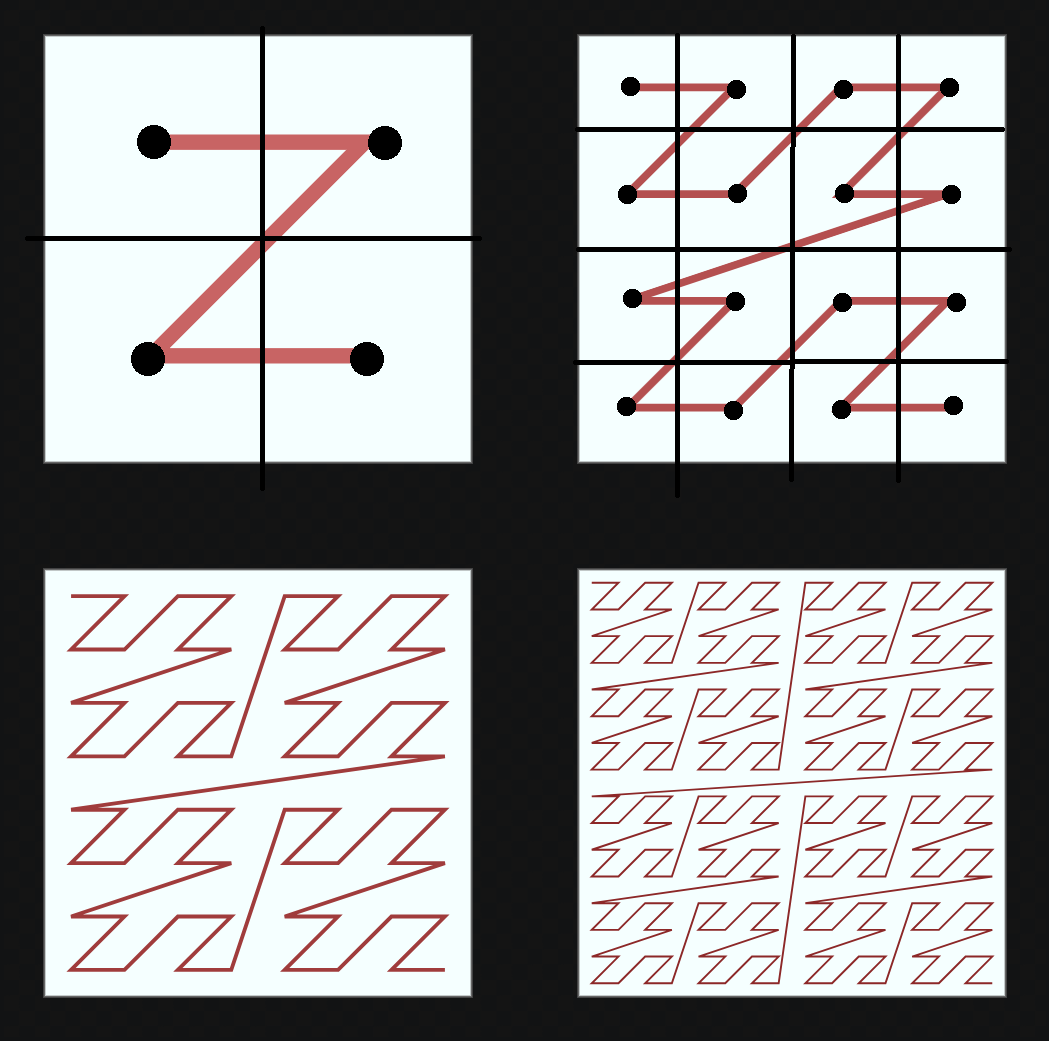
\includegraphics[width=0.45\textwidth]{./Z-morton_grid.png}

    \underline{\textbf{Avantages :}} \\
    Proximité en mémoire $\rightarrow$  Rapidité de calcul 

    \vspace{3mm}

    \underline{\textbf{Inconvénients :}} \\
    Grille carré \\
    Taille en puissance de 2

    \end{center}
\end{frame}

\begin{frame}{Parall    élisation}   
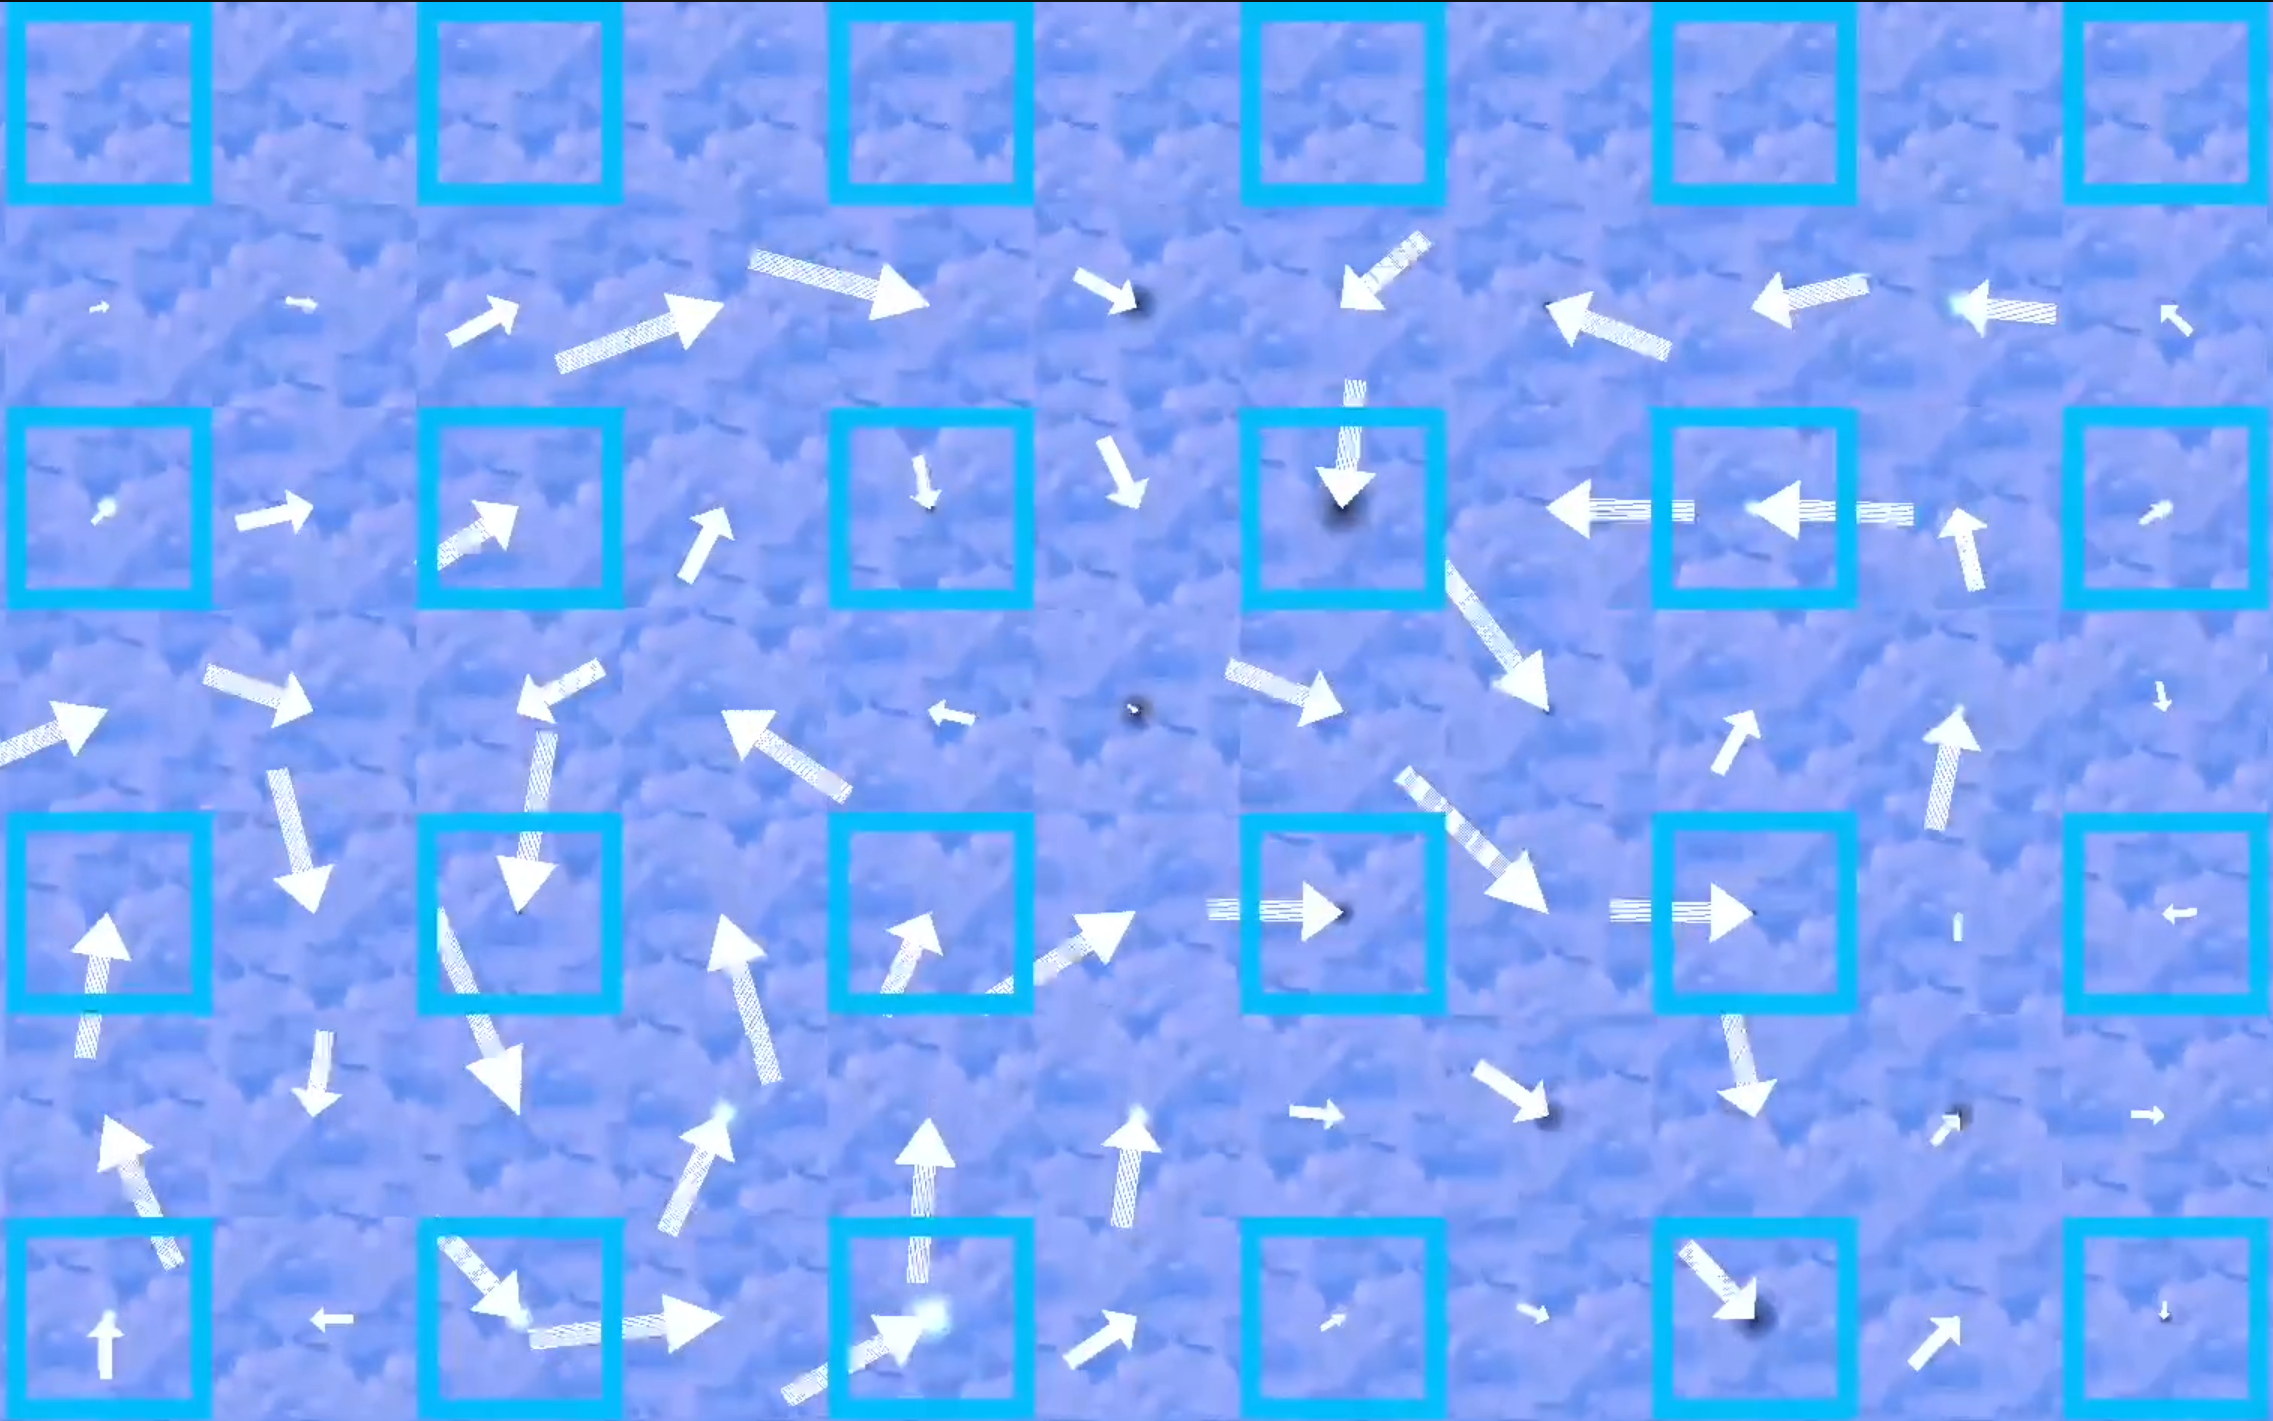
\includegraphics[width=1\textwidth]{./Parralélisation.png}
\end{frame}

\begin{frame}{Features}  
    Tracer des murs et des objets solides à chaud\\
    \vspace{0.5cm}
    \begin{columns}[c]
    % --- Colonne de gauche ---
    \begin{column}{0.48\textwidth}
        \centering
        \fbox{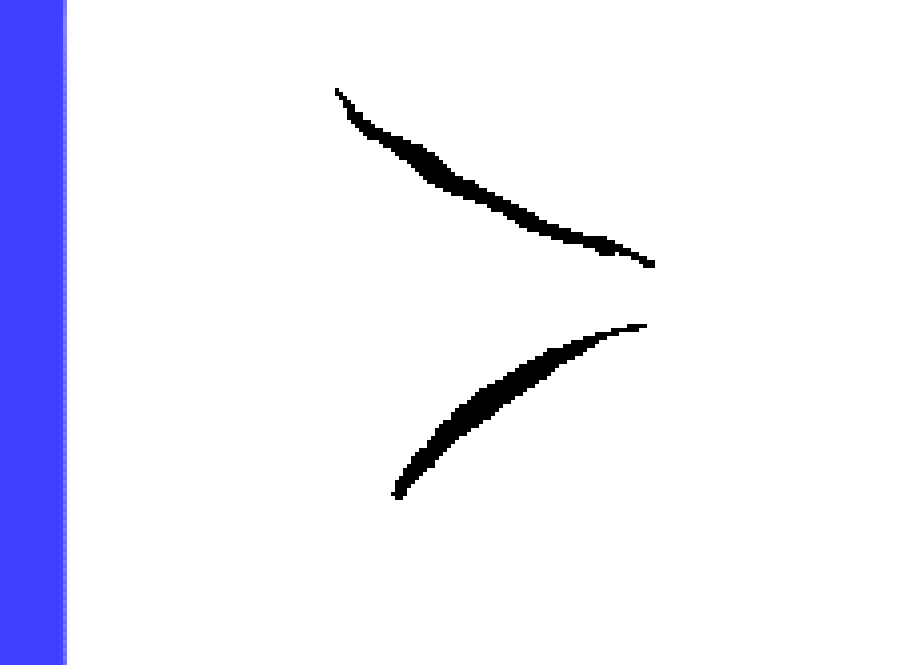
\includegraphics[width=0.8\textwidth]{./Dessin (3).png}}
        \fbox{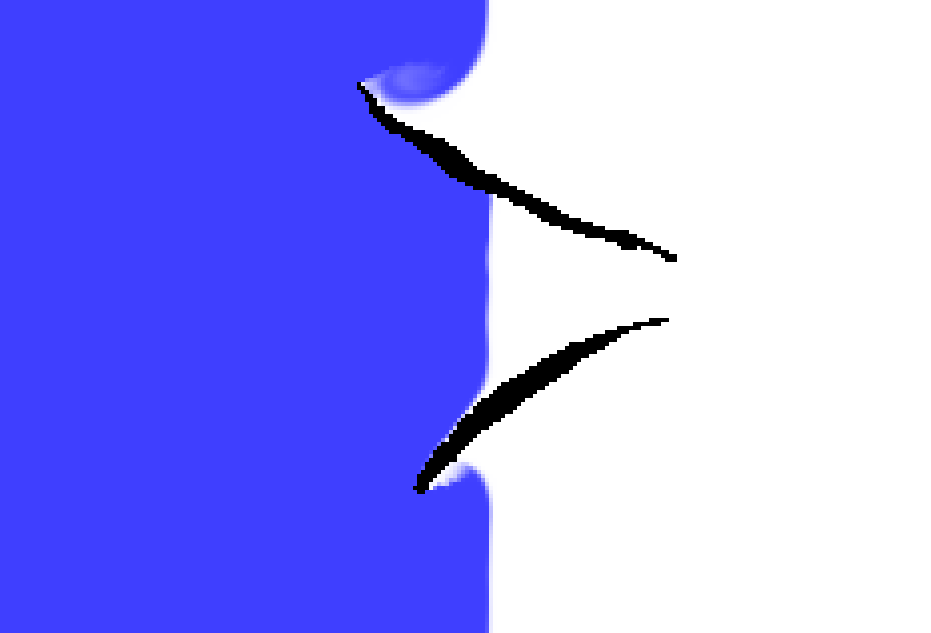
\includegraphics[width=0.8\textwidth]{./Dessin (2).png}}
    \end{column}
    % --- Séparateur vertical ---
    \begin{column}{0.01\textwidth}
        \centering
        \begin{tikzpicture}
            \draw[very thick,gray!60] (0,0) -- (0,5);
        \end{tikzpicture}
    \end{column}
    % --- Troisième image ---
    \begin{column}{0.48\textwidth}
        \centering
        \fbox{
\includegraphics[width=1\textwidth]{./Dessin (1).png}}
    \end{column}
    \end{columns}
\end{frame}

\begin{frame}{Capacités du solveur}

\textbf{Exemples}

\vspace{0.2cm}

\begin{columns}[c]

    % --- Colonne de gauche ---
    \begin{column}{0.48\textwidth}
        \centering
        \fbox{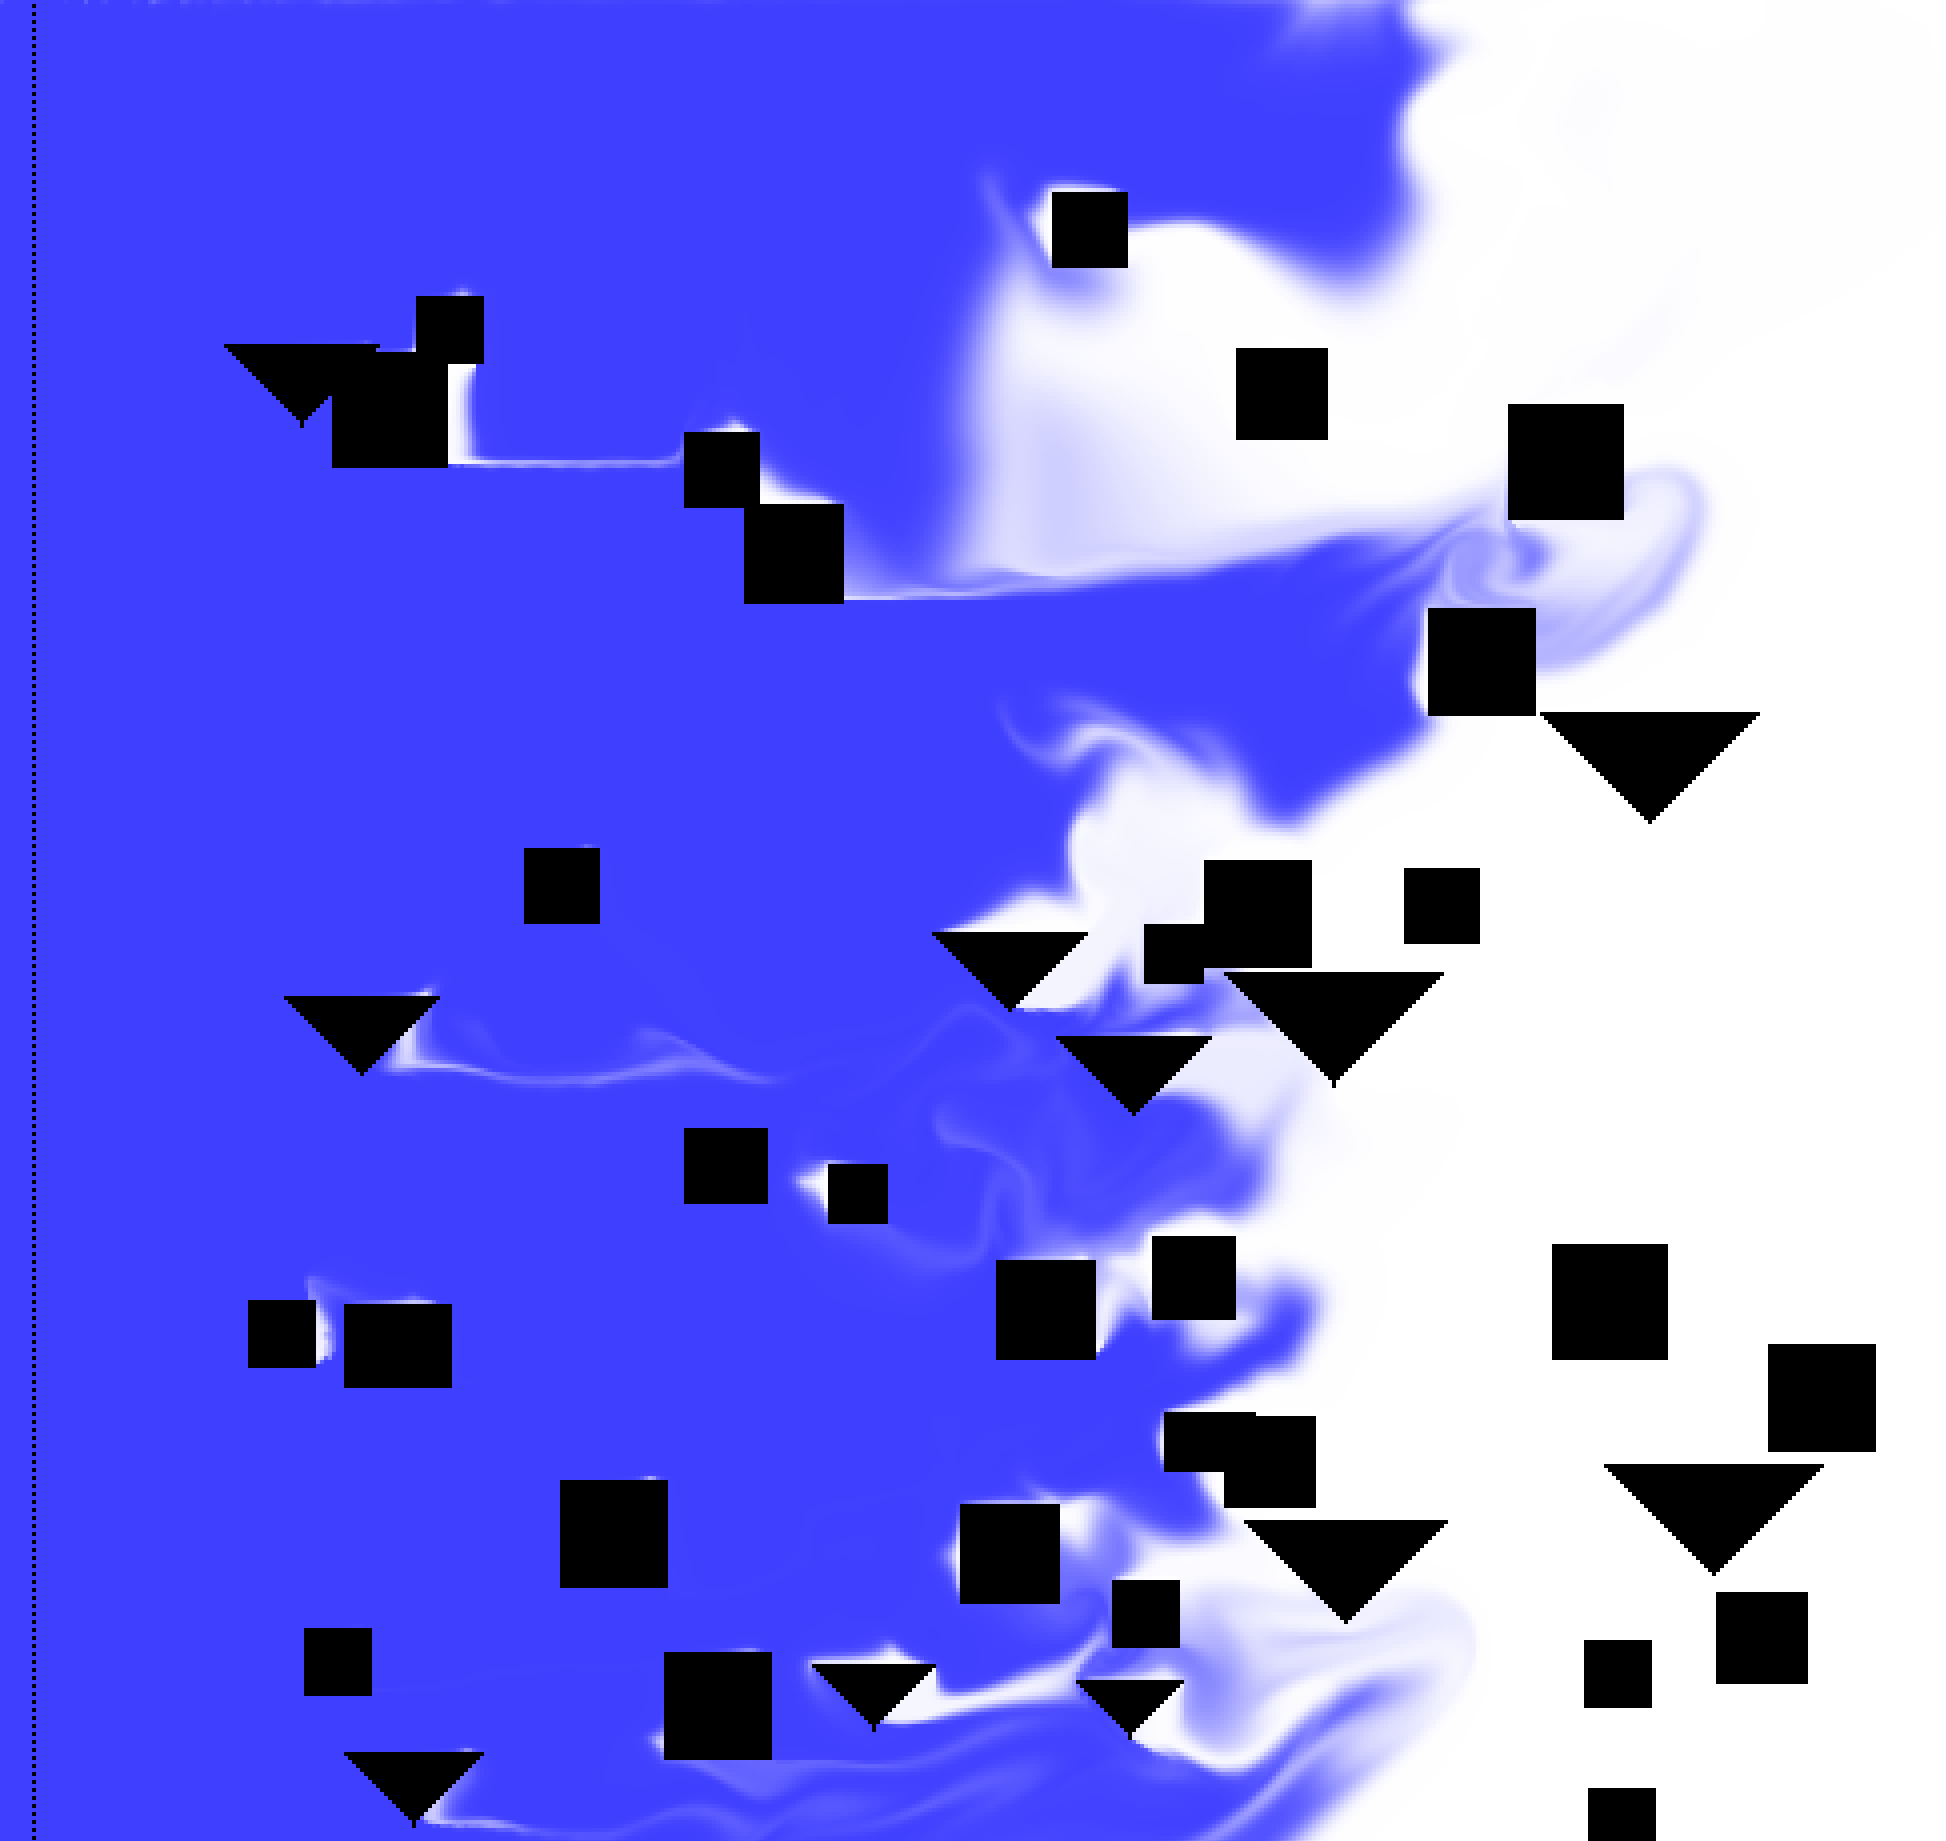
\includegraphics[width=0.9\textwidth]{city_simulation.png}}
    \end{column}

    % --- Séparateur vertical ---
    \begin{column}{0.01\textwidth}
        \centering
        \begin{tikzpicture}
            \draw[very thick,gray!60] (0,0) -- (0,5);
        \end{tikzpicture}
    \end{column}

    % --- Colonne de droite ---
    \begin{column}{0.48\textwidth}
        \centering
        \fbox{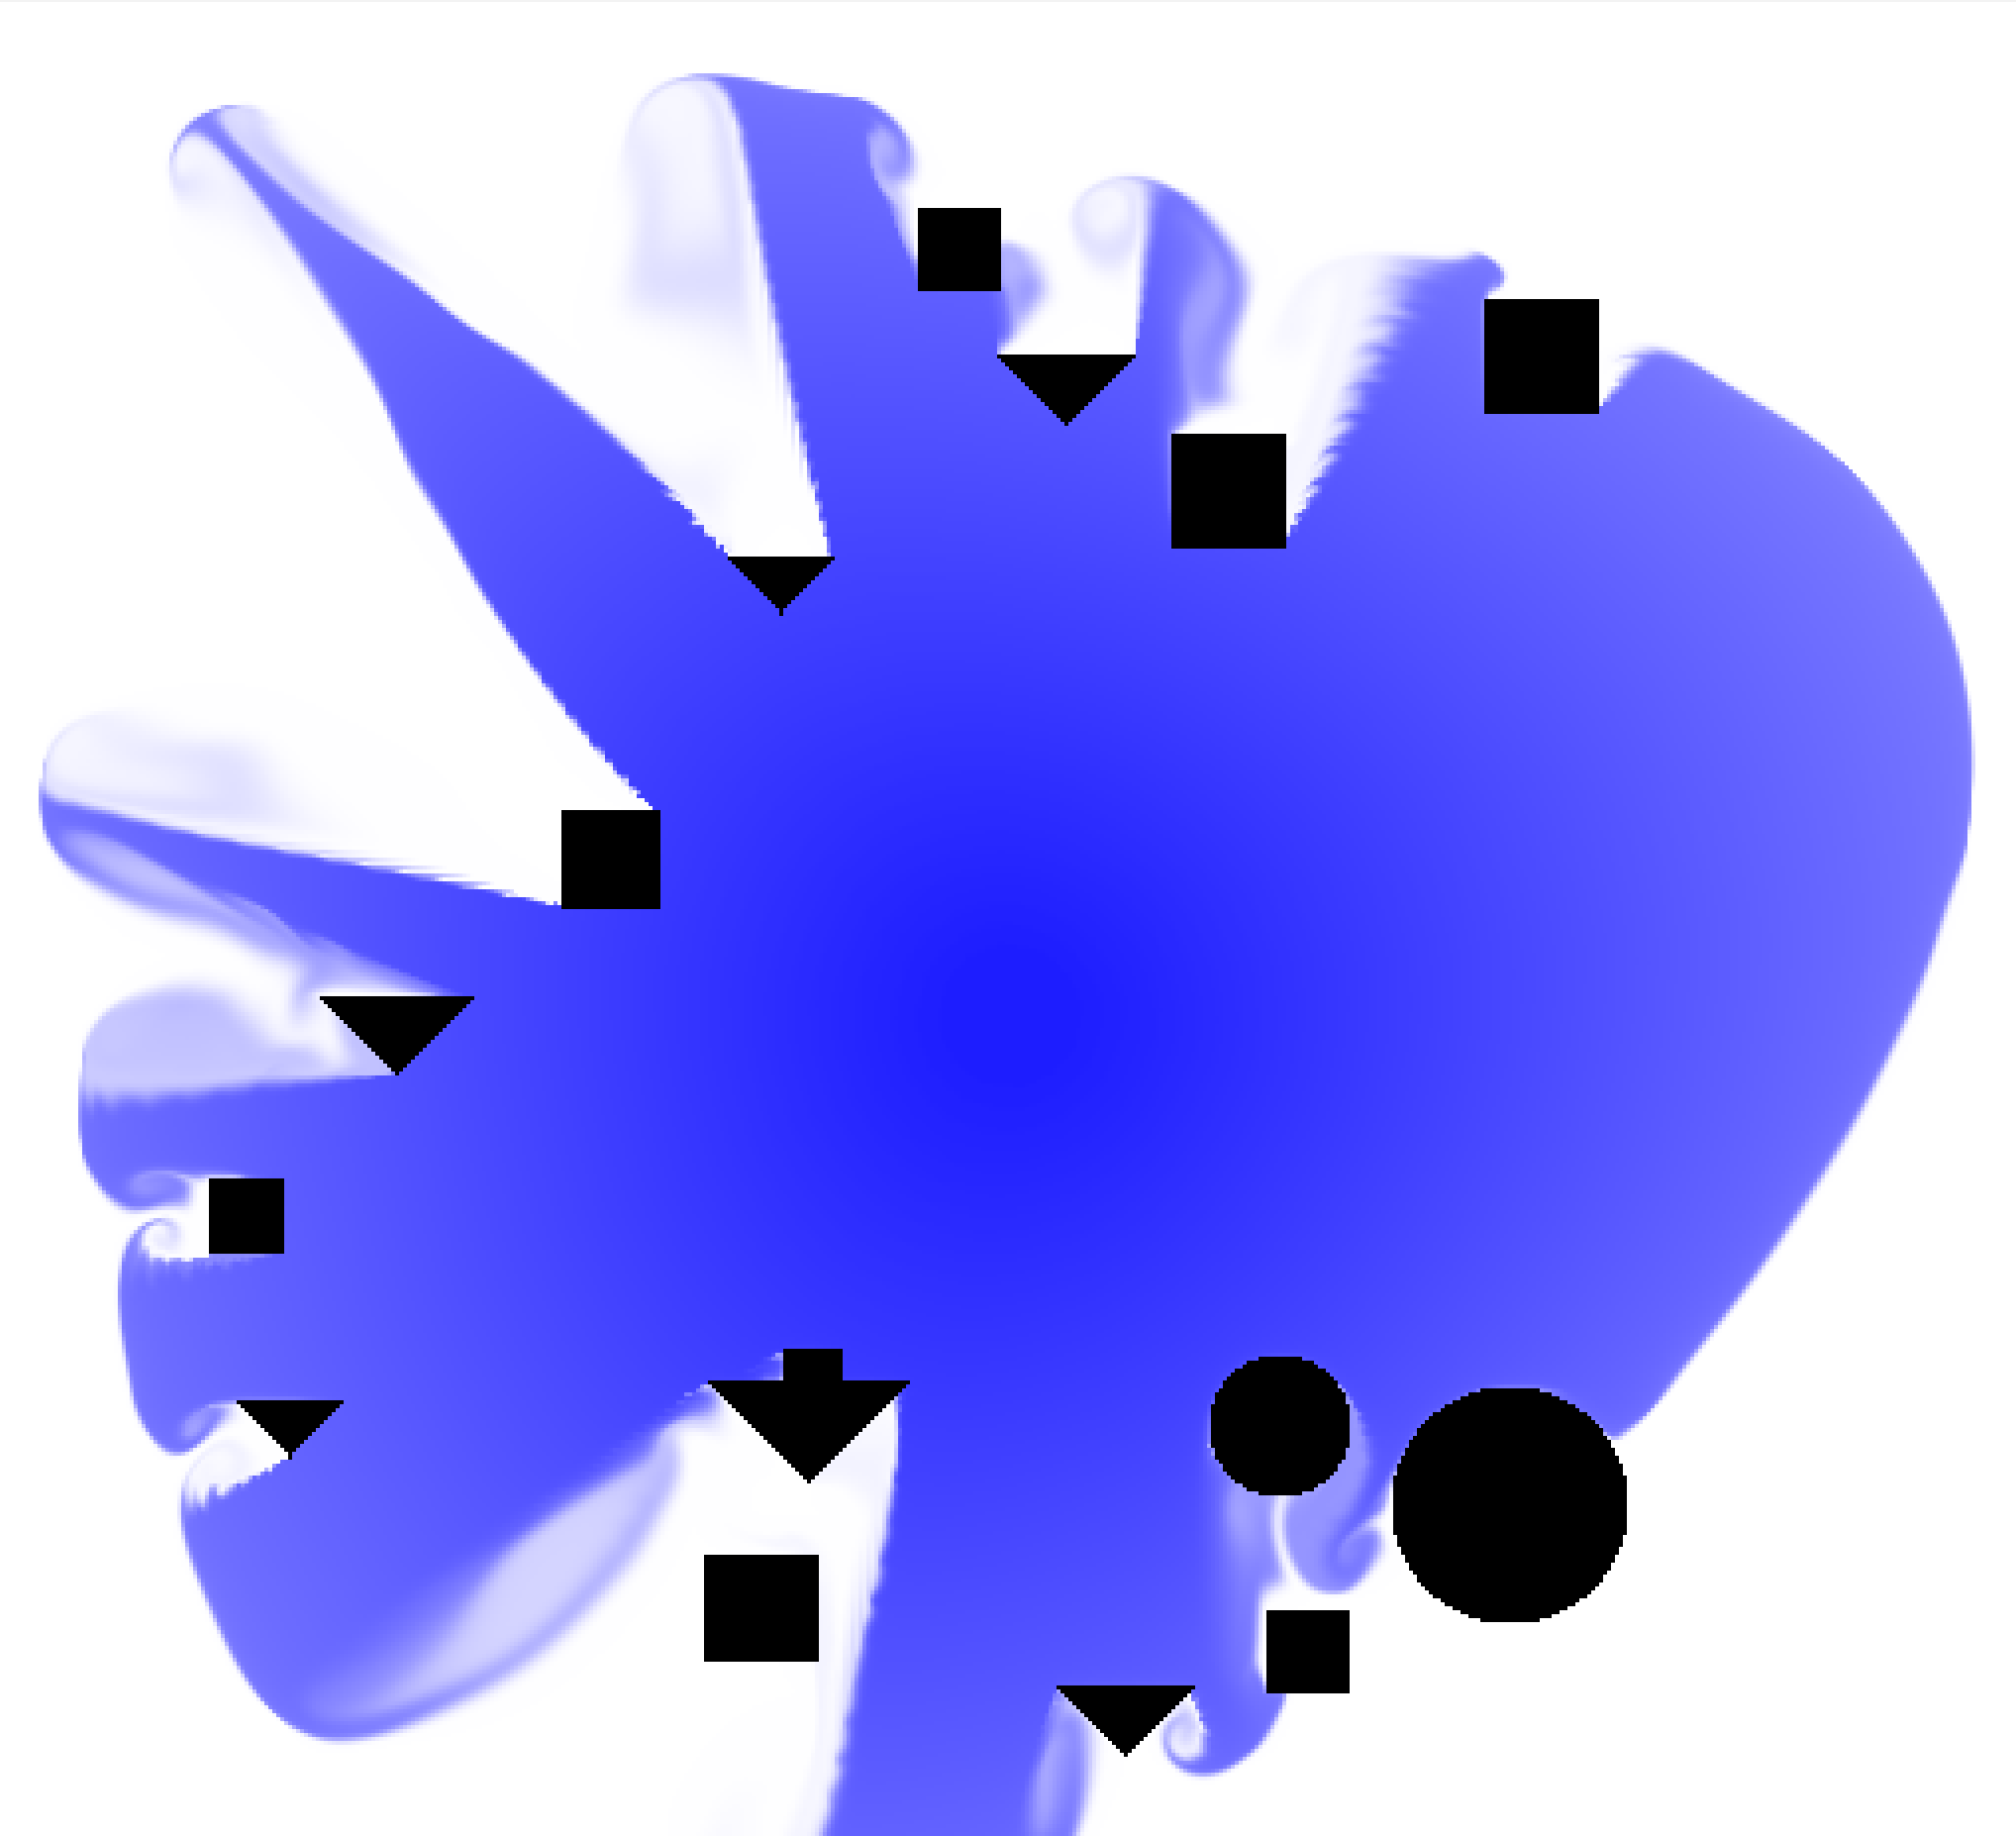
\includegraphics[width=1.0\textwidth]{center_source.png}}
    \end{column}

\end{columns}

\end{frame}

\begin{frame}{Vortex}
\vspace{-1.5cm}
\Large \textbf{}\\
\vspace{0.5cm}

\includegraphics[width=1\textwidth]{./vortex_zip/ezgif-frame-005.png}
\end{frame}

\begin{frame}{Vortex de Von Karman}
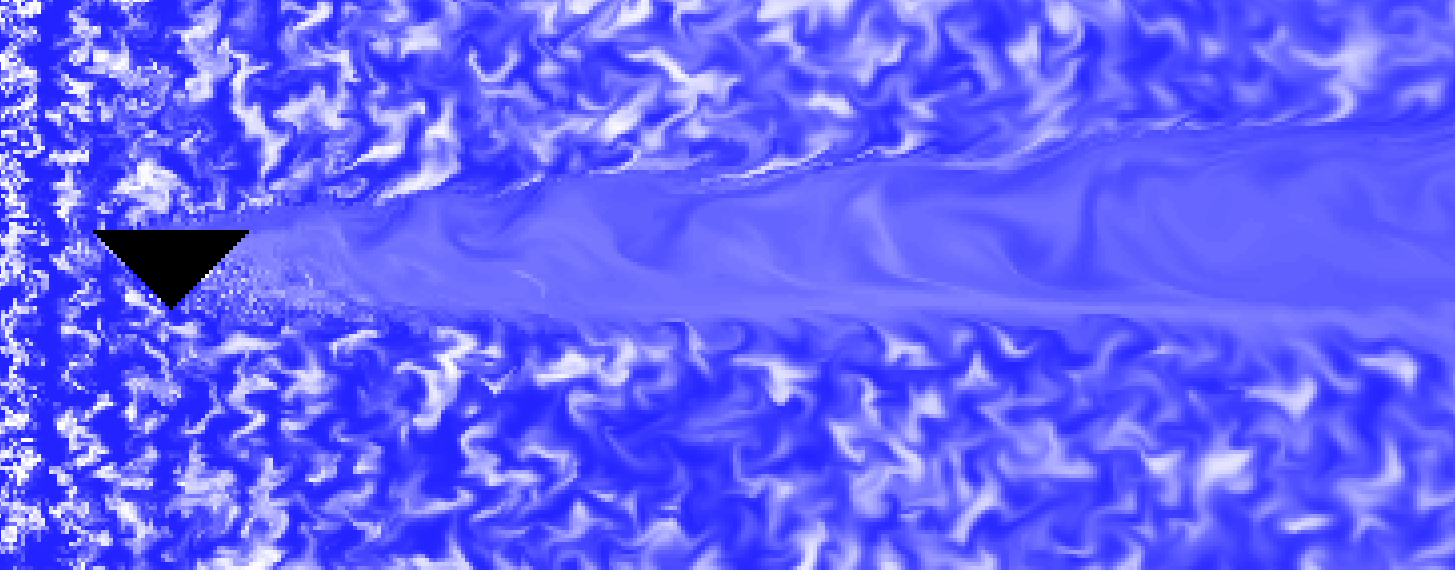
\includegraphics[width=1\textwidth]{./Von Karman (3).png}
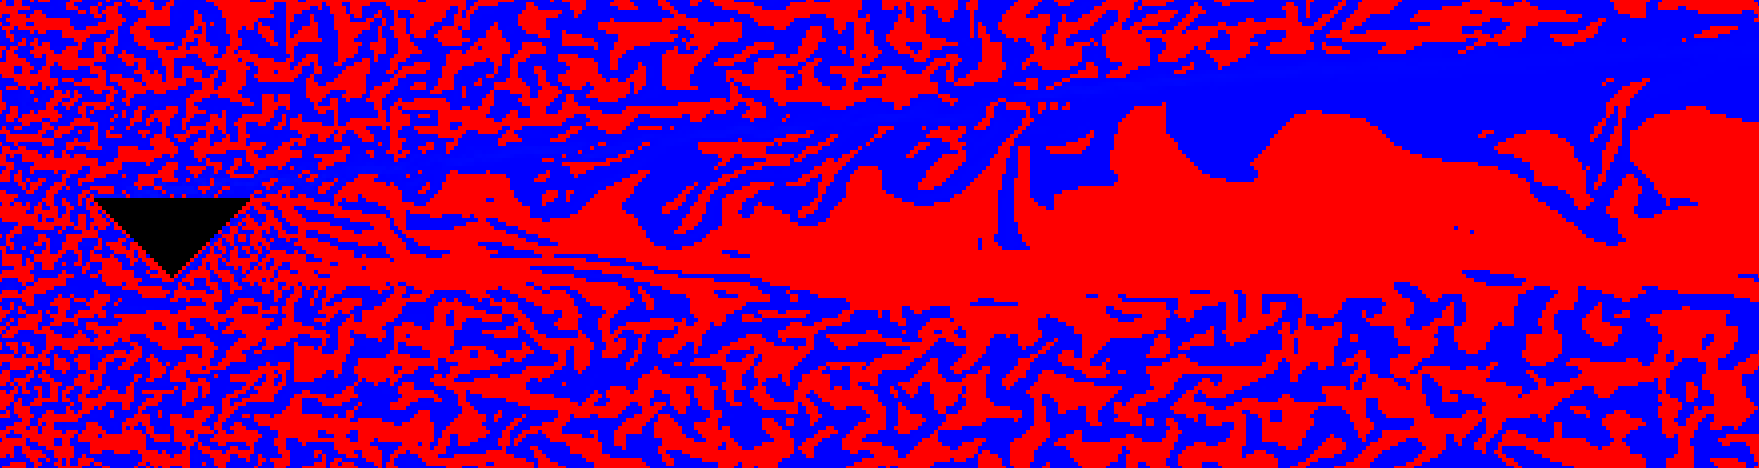
\includegraphics[width=1\textwidth]{./Von Karman (1).png}
\end{frame}

\begin{frame}{Méthode de calcul des forces}
\small
\begin{itemize}
    \item[$\bullet$] \textbf{compute\_walls\_forces} : force par cellule mur
        \begin{itemize}
            \item[$\circ$] Pour chaque mur, examine les voisins fluides
            \item[$\circ$] Calcule 3 forces : pression (normale), traînée (opposée à la vitesse), cisaillement (tangentiel)
        \end{itemize}

    \item[$\bullet$] \textbf{identify\_objects} : identification des objets
        \begin{itemize}
            \item[$\circ$] Pour les murs non marqués, lance un DFS
            \item[$\circ$] ID attribués aux murs des objets connexes
        \end{itemize}

    \item[$\bullet$] \textbf{compute\_object\_forces} : calcul forces et moments
        \begin{itemize}
            \item[$\circ$] Premier passage : accumule les forces et calcule le centre de masse de chaque objet
            \item[$\circ$] Second passage : calcule moment de force via le produit vectoriel 2D
            \item 
            \begin{center} 
                \vspace{0.2cm}
                $\overrightarrow{\mathcal{M}_o} = \overrightarrow{OM} \wedge \overrightarrow{F}$ 
            \end{center}
        \end{itemize}
\end{itemize}

\end{frame}

\begin{frame}{Forces et optimisation de structures }
    \begin{center}
        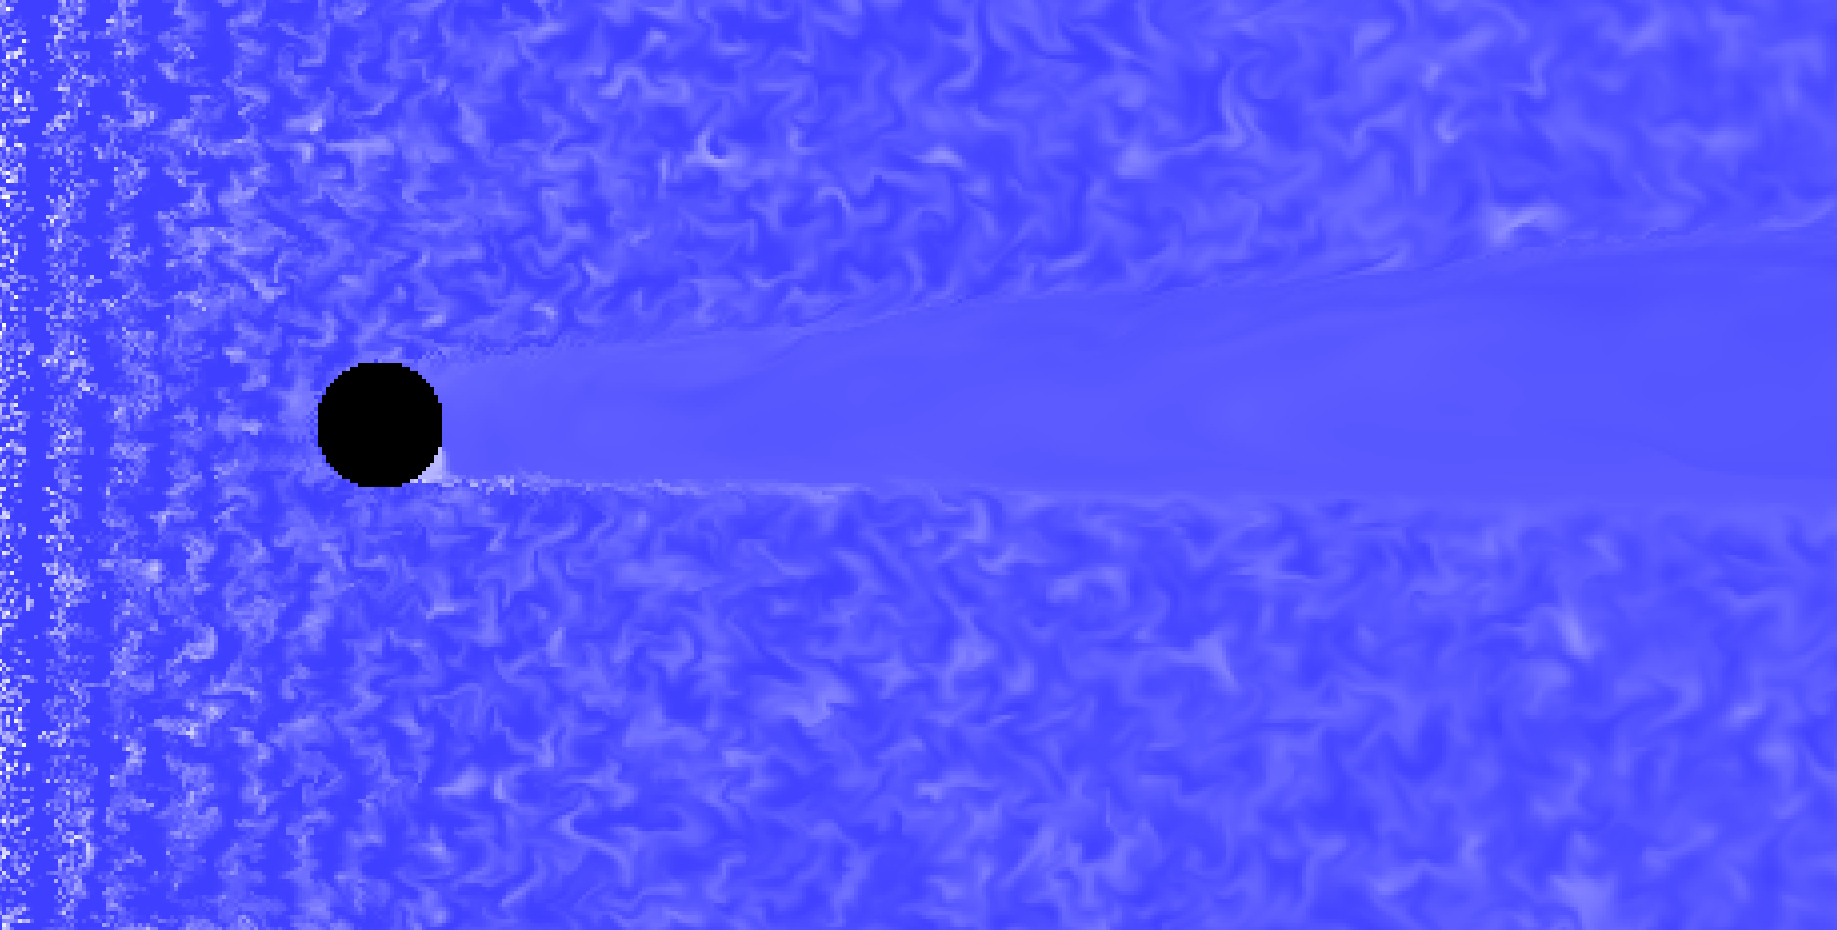
\includegraphics[width=1\textwidth]{./Trainée_cercle_1.png}
    \end{center}
\end{frame}
    
\begin{frame}{Forces et optimisation de structures }   

\begin{columns}[c]
    \begin{column}{0.55\textwidth}
        \centering
        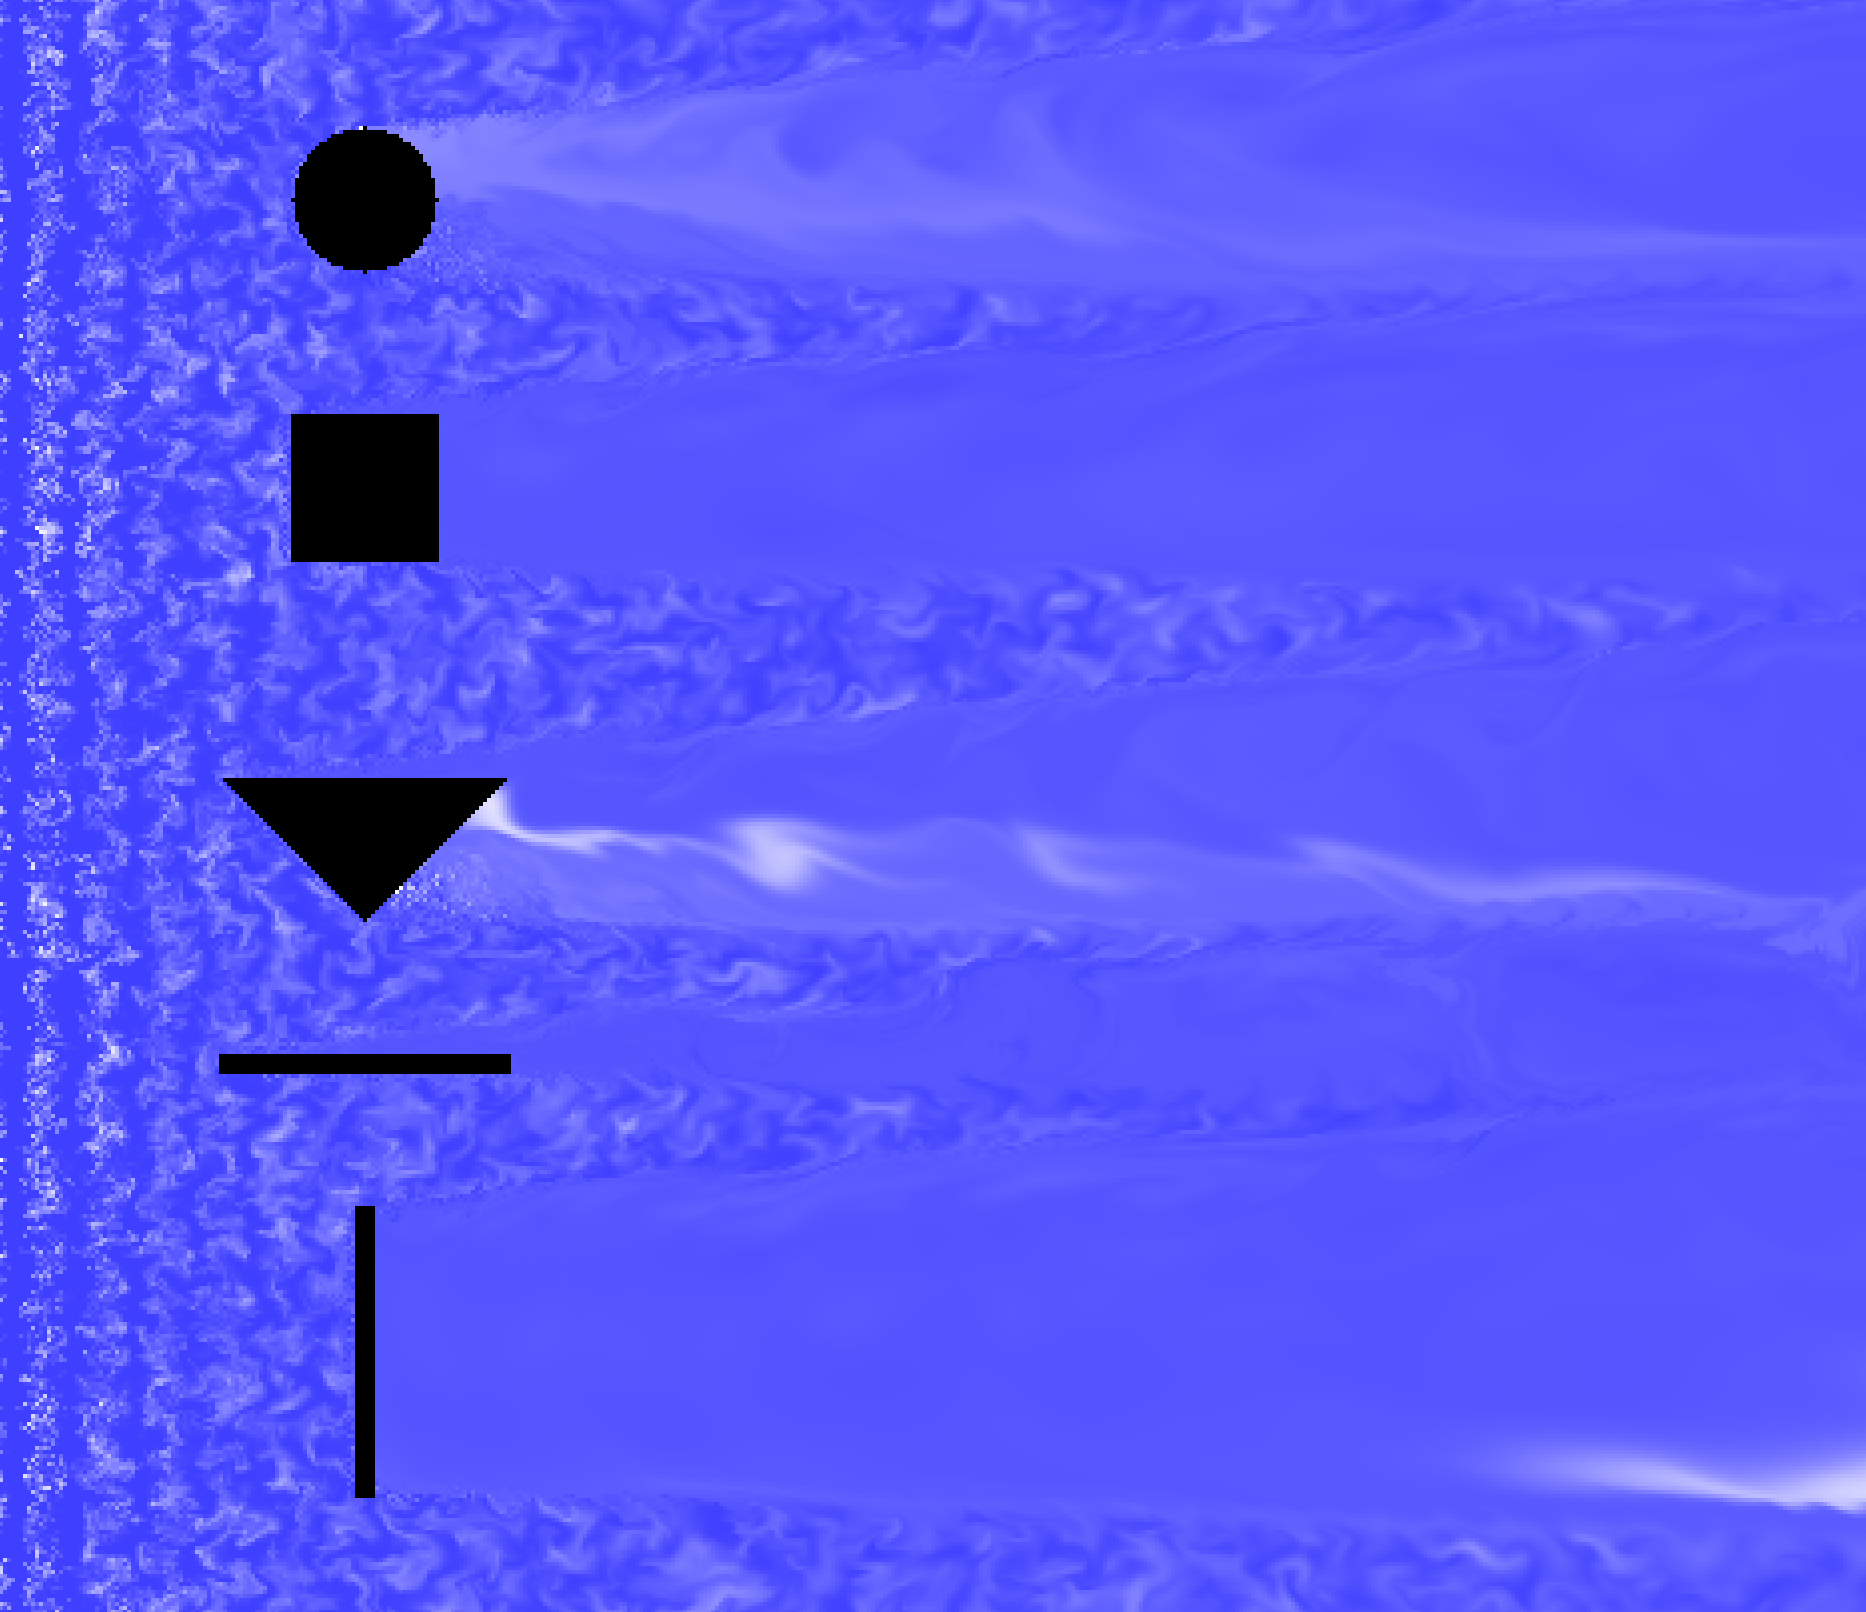
\includegraphics[width=0.98\textwidth]{./trainées 1.png}
    \end{column}
    \begin{column}{0.53\textwidth}
        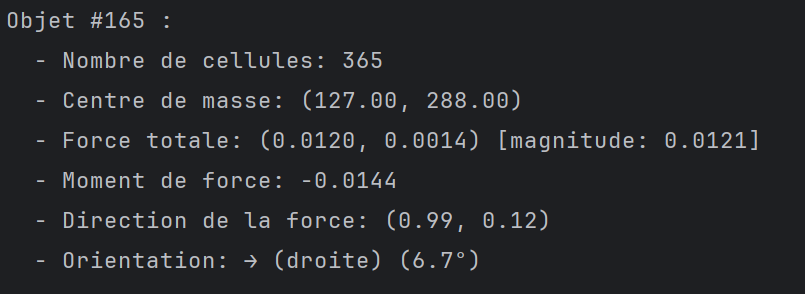
\includegraphics[width=1.0\textwidth]{./object_forces.png}
    \end{column}
\end{columns}

\end{frame}

\begin{frame}{Forces et optimisation de structures }   

\begin{columns}[c]
    \begin{column}{0.5\textwidth}
        \centering
        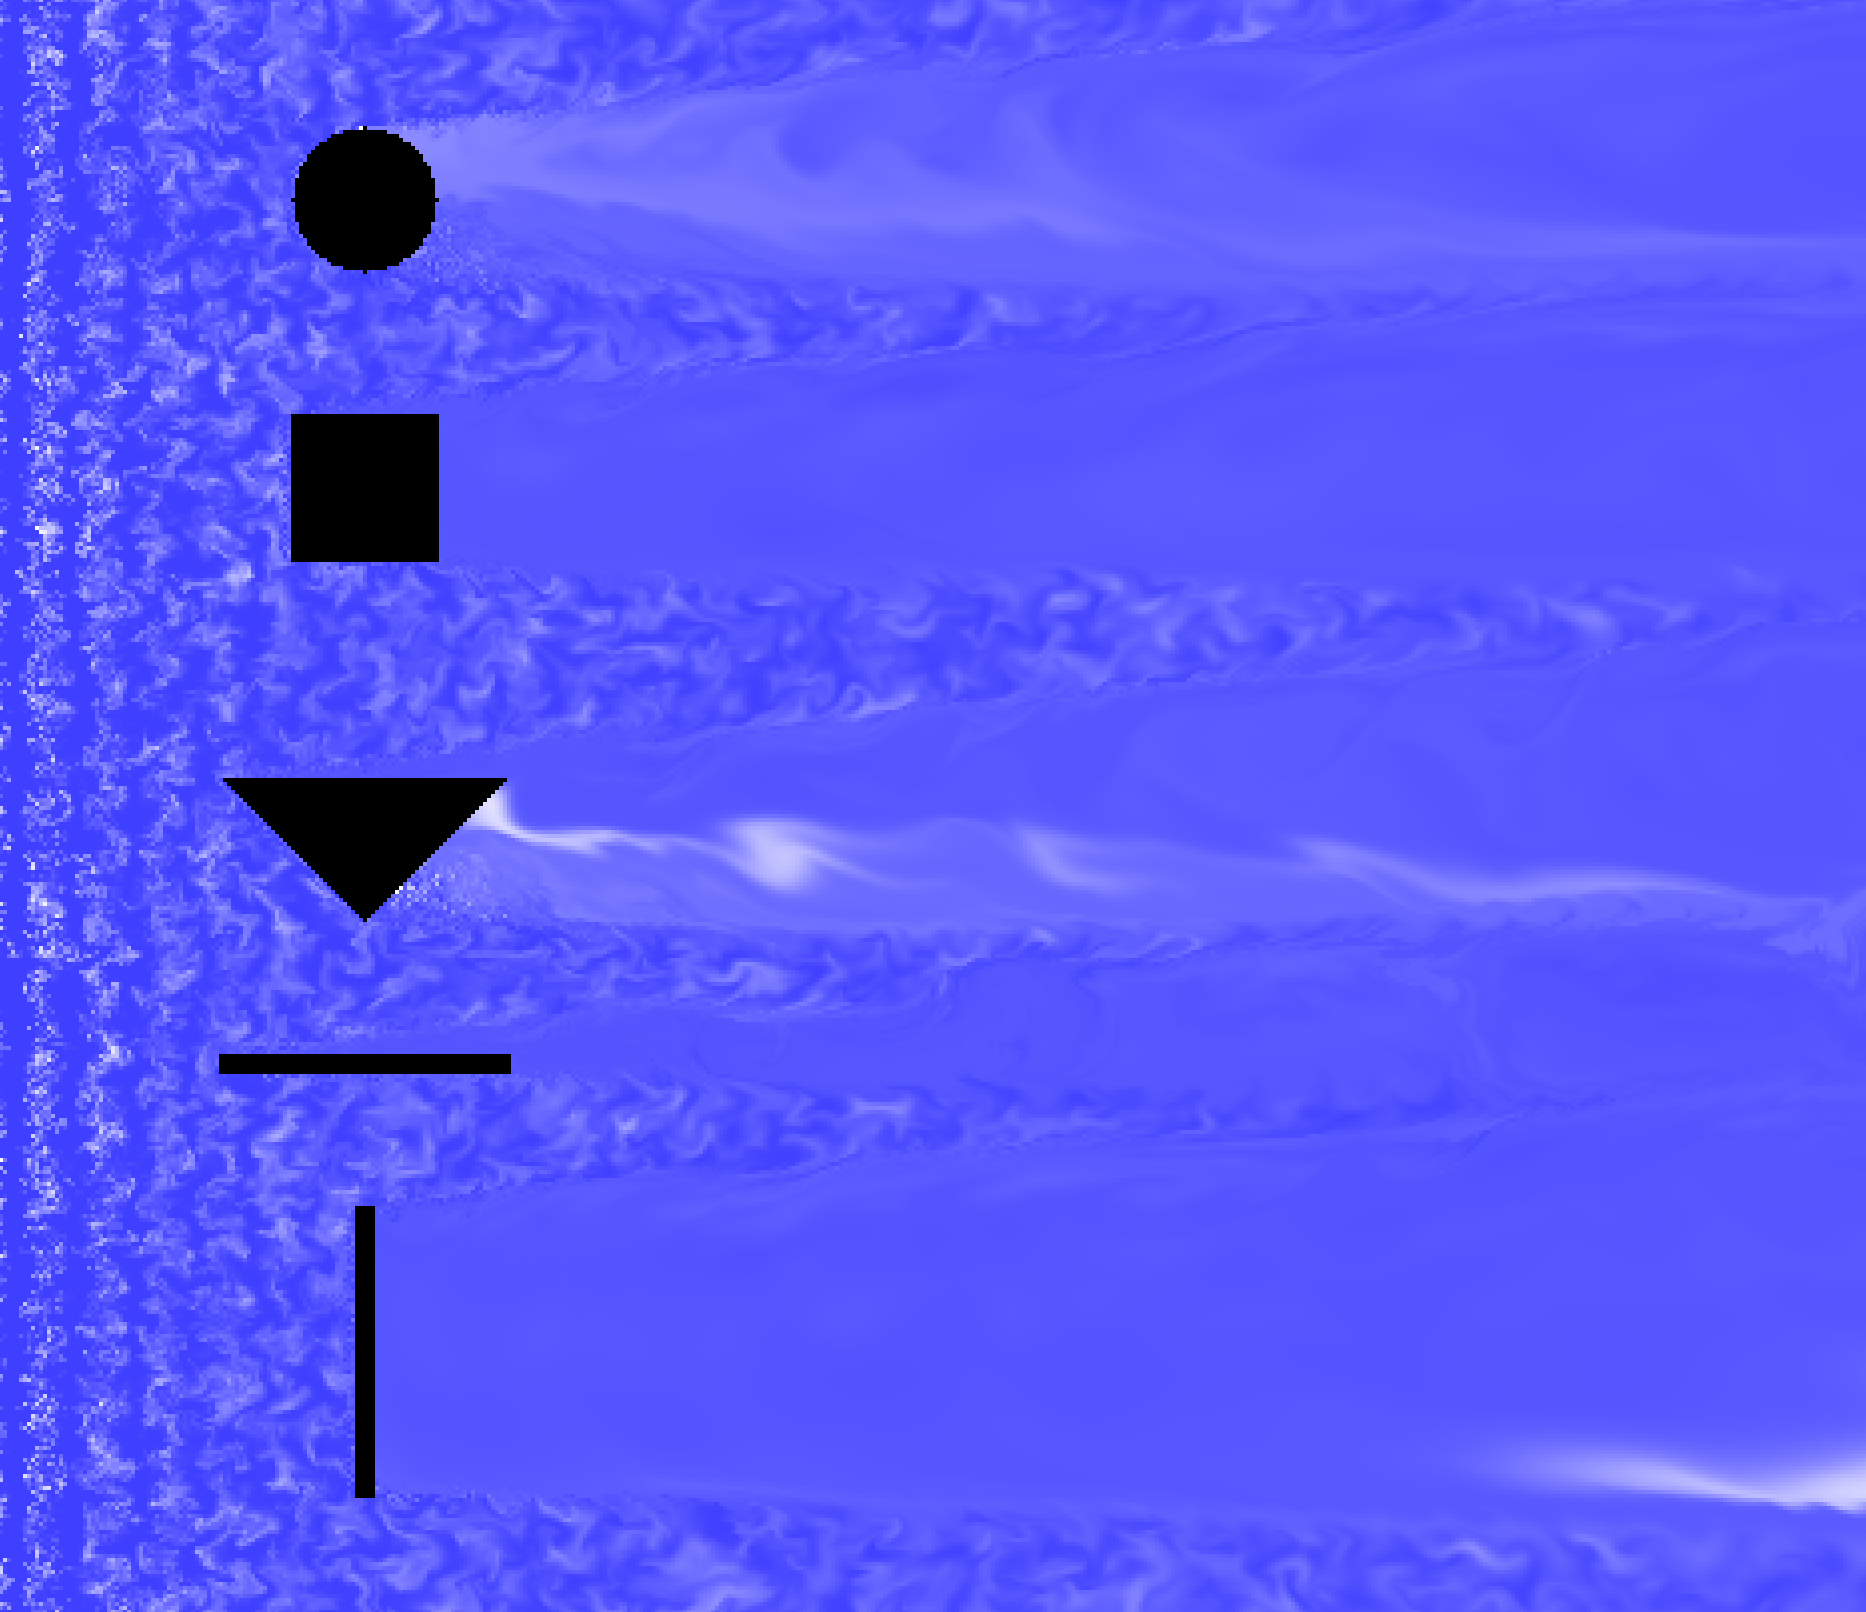
\includegraphics[width=1.099\textwidth]{./trainées 1.png}
    \end{column}
    \begin{column}{0.5\textwidth}
        \centering
        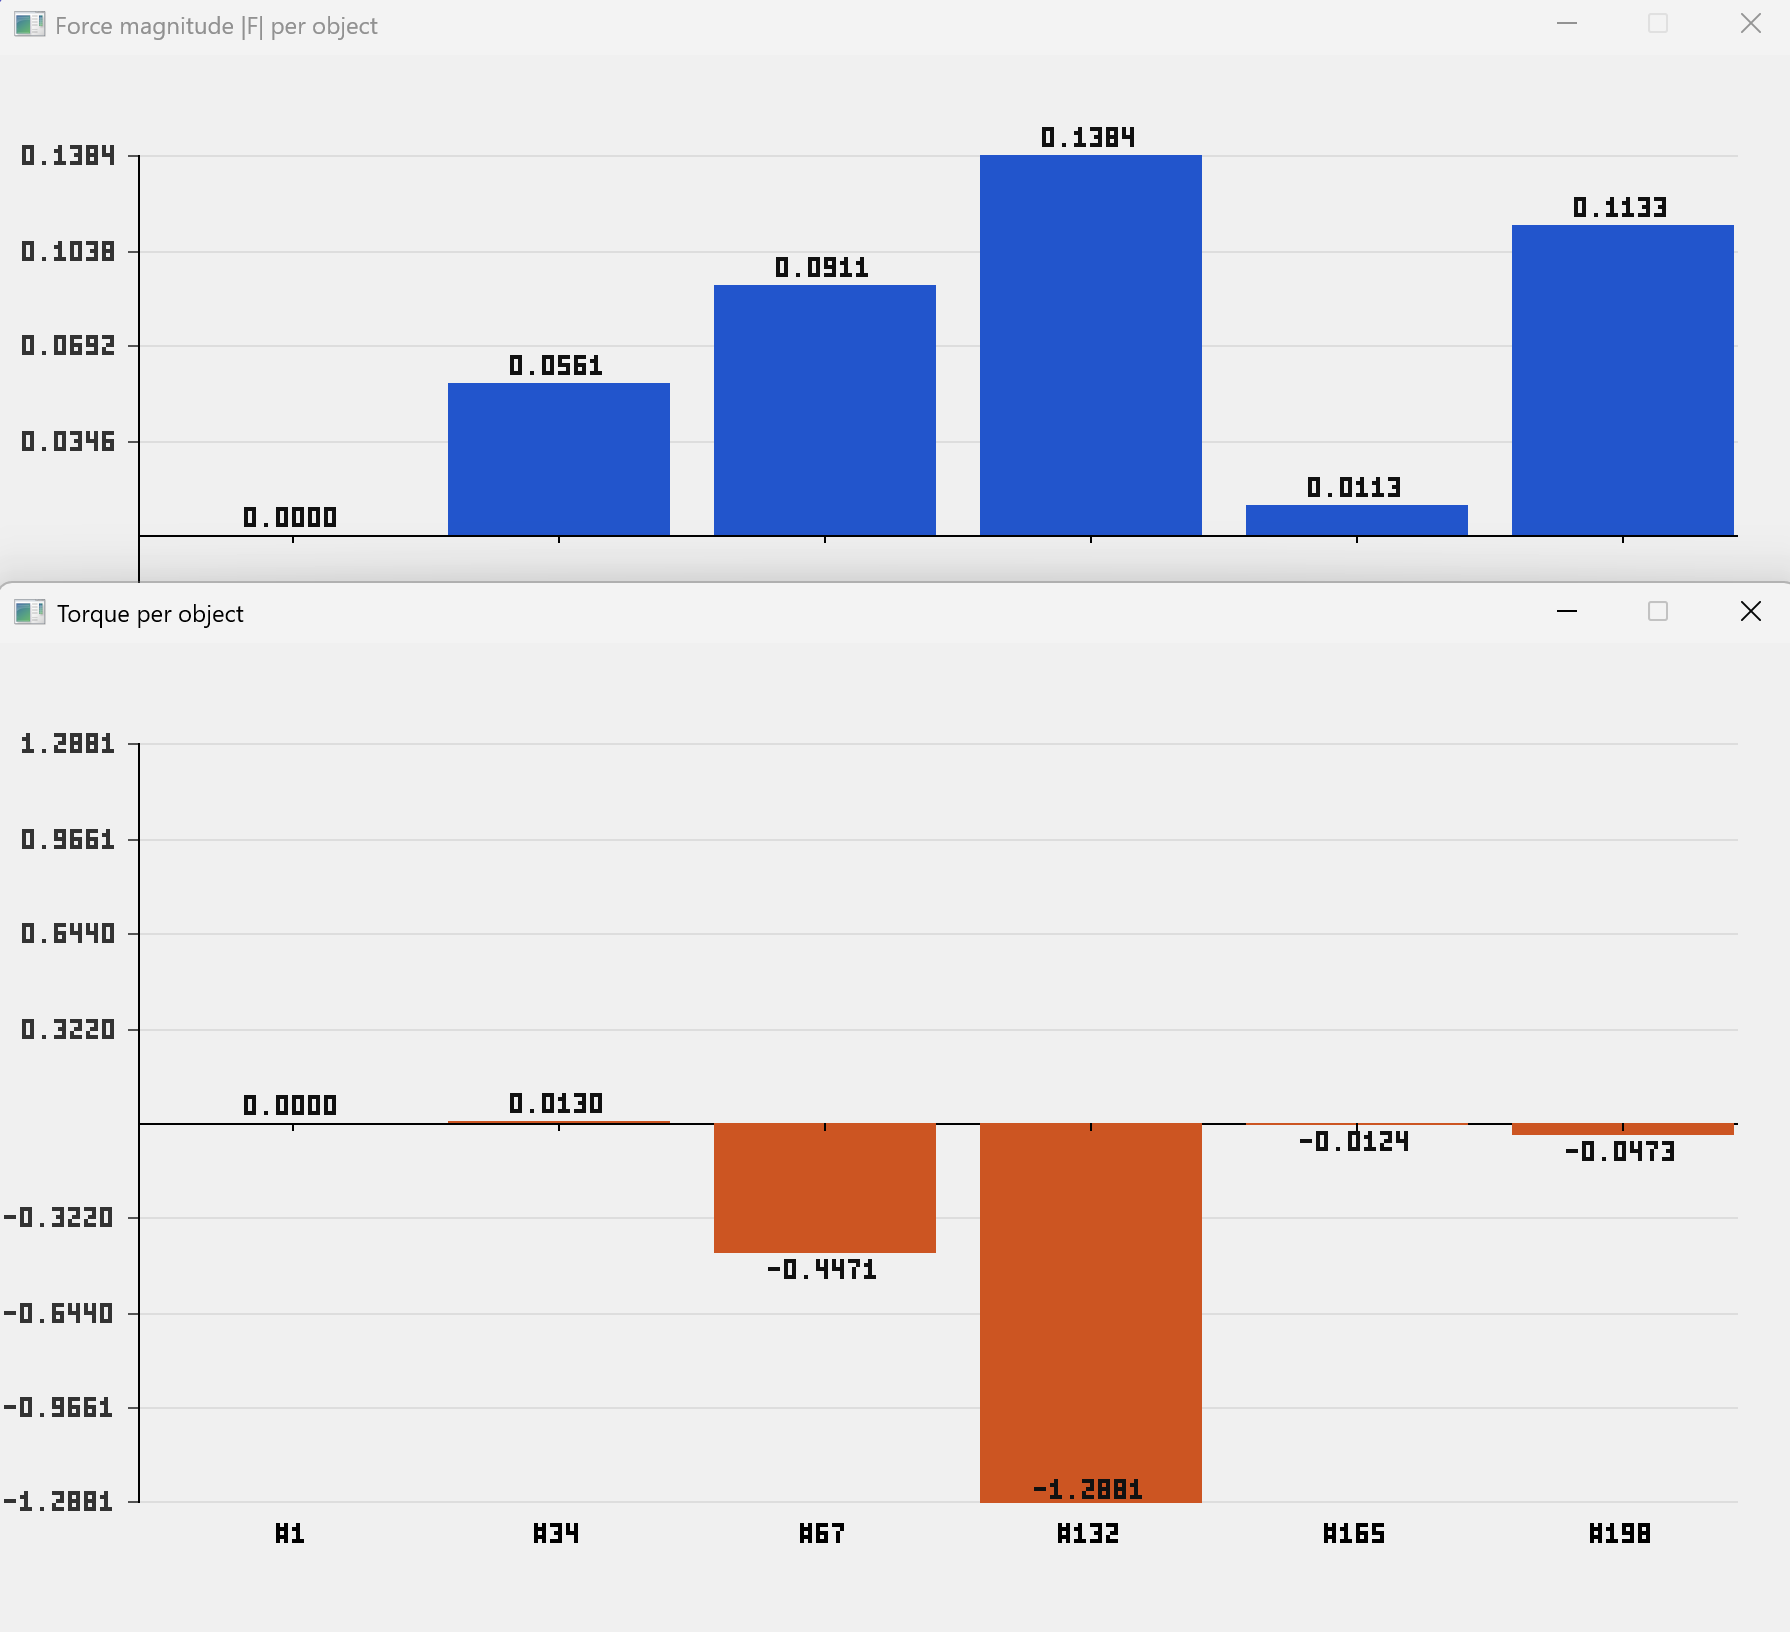
\includegraphics[width=1.04\textwidth]{./Torque_and_force_graph (5).png}
    \end{column}
\end{columns}

\end{frame}
\begin{frame}{Forces et optimisation de structures }    
    \begin{center}
        \begin{columns}[c]
            \setlength{\columnsep}{0.15cm}
            \begin{column}{0.48\textwidth}
                \centering
                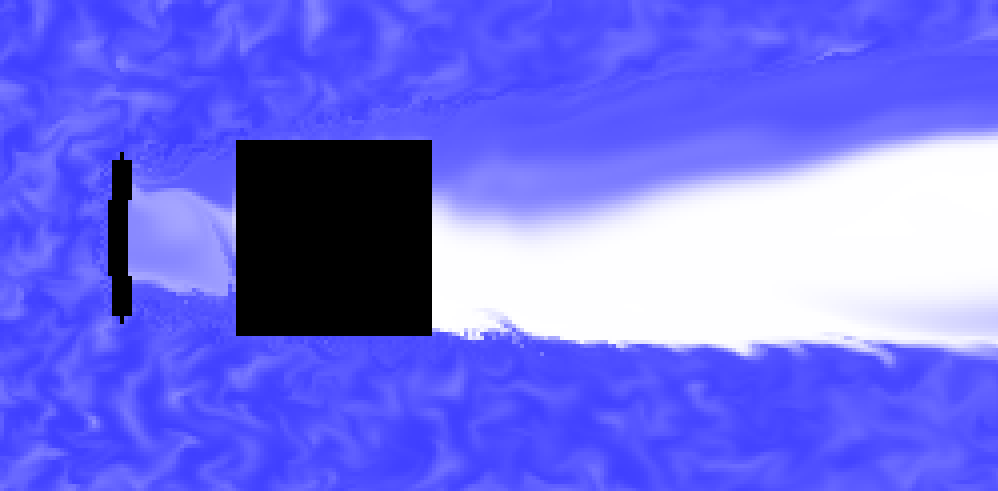
\includegraphics[width=0.8\textwidth]{./test_protection (1).png}

                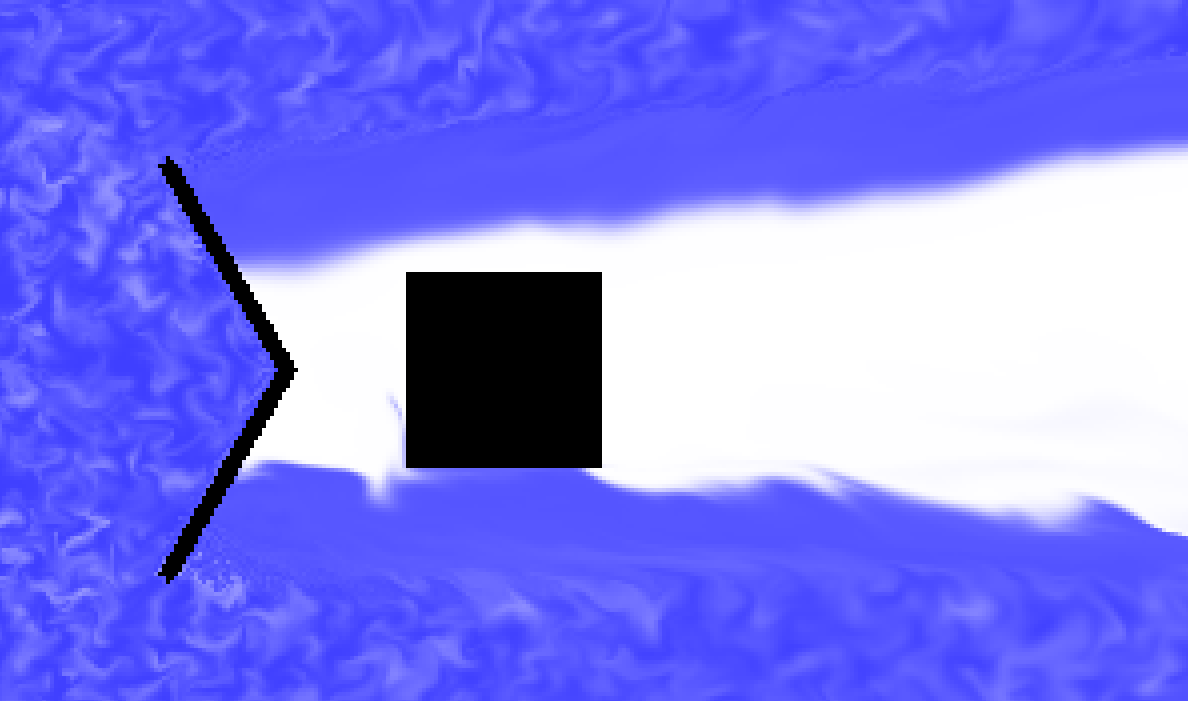
\includegraphics[width=0.8\textwidth]{./test_protection (3).png}

                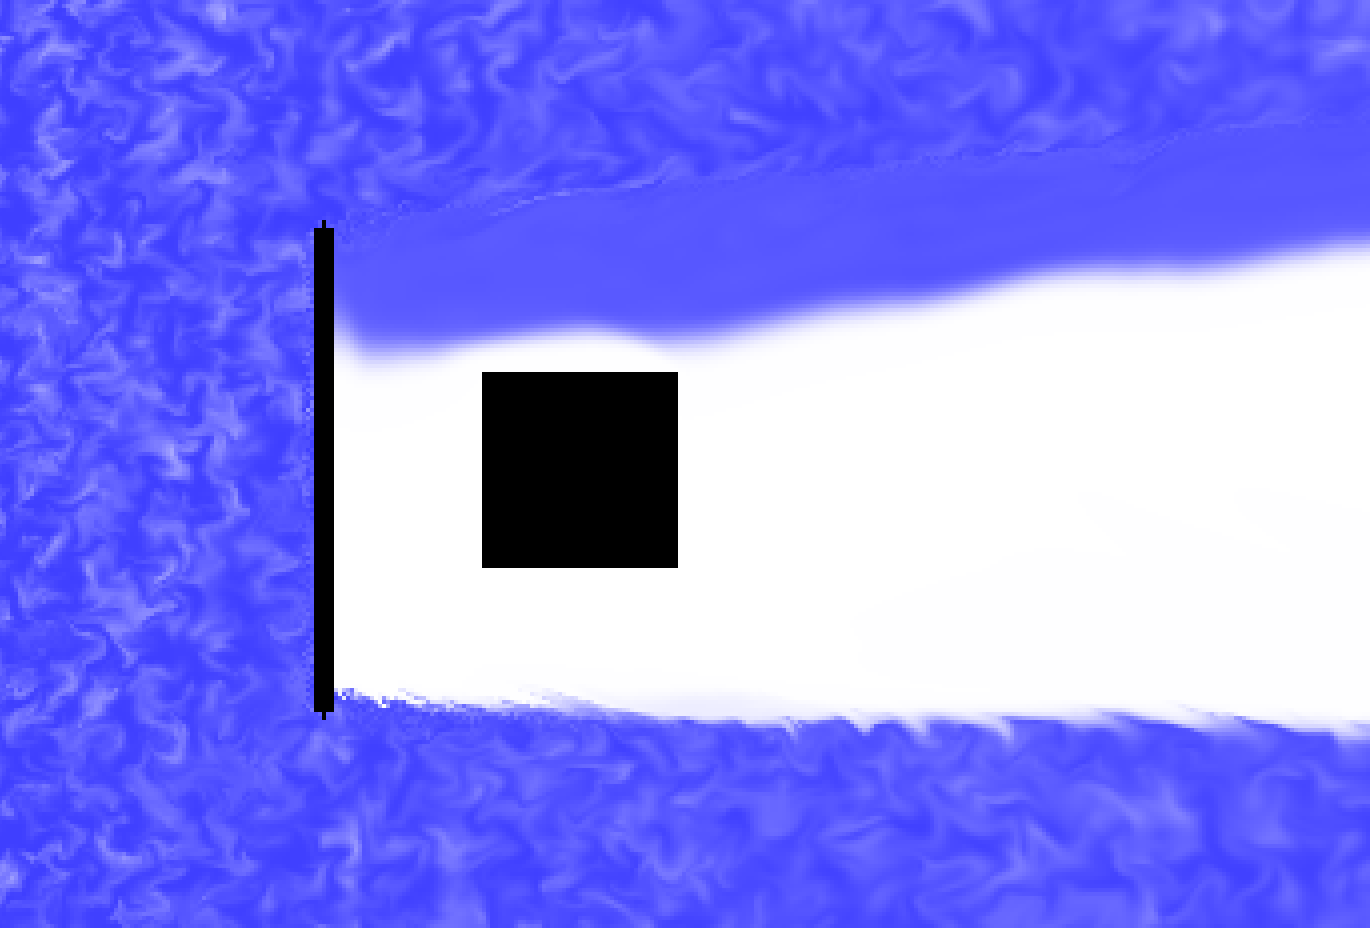
\includegraphics[width=0.8\textwidth]{./test_protection (5).png}
            \end{column}

            \begin{column}{0.48\textwidth}
                \centering
                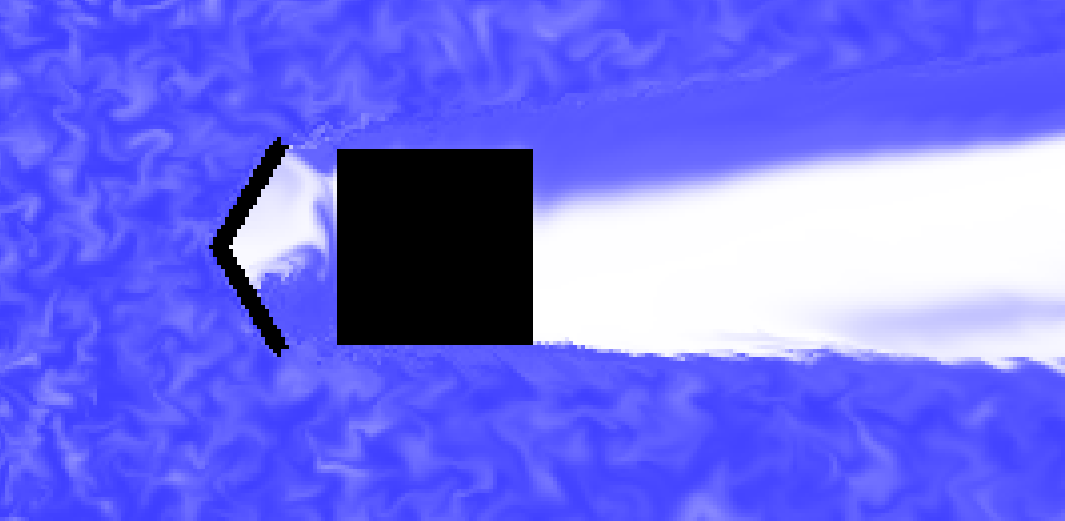
\includegraphics[width=0.8\textwidth]{./test_protection (2).png}

                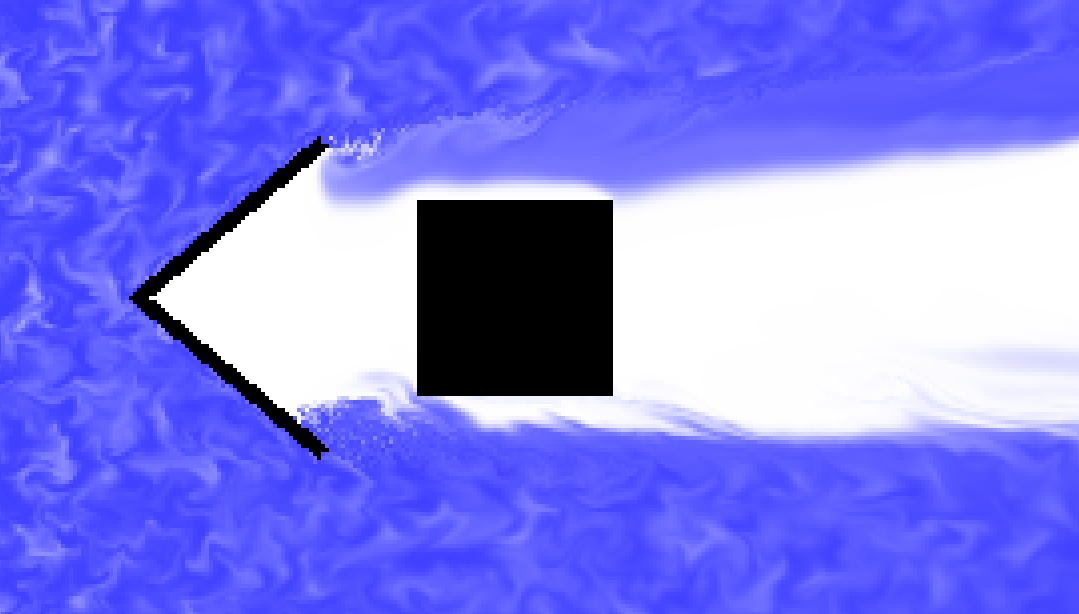
\includegraphics[width=0.8\textwidth]{./test_protection (4).png}

                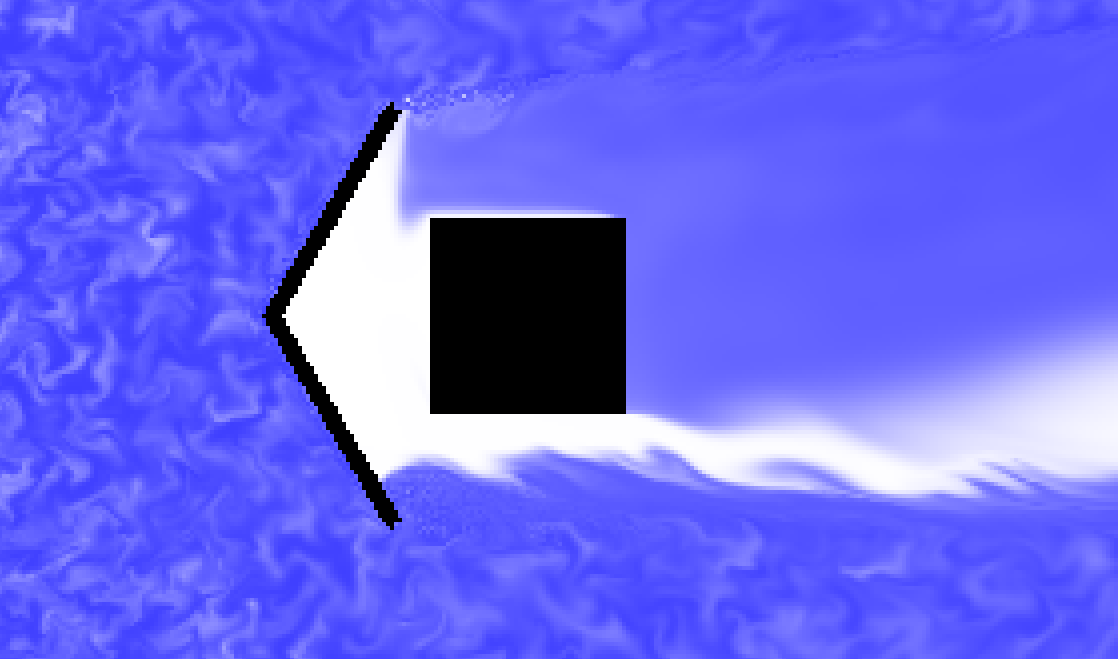
\includegraphics[width=0.8\textwidth]{./test_protection (6).png}
                
                \vspace{0.3cm}
            \end{column}
        \end{columns}
    \end{center}
\end{frame}

\begin{frame}{}
\textbf{Problèmes}\\
    \begin{columns}[c]

    % --- Colonne de gauche ---
    \begin{column}{0.48\textwidth}
        \centering
        \boxed{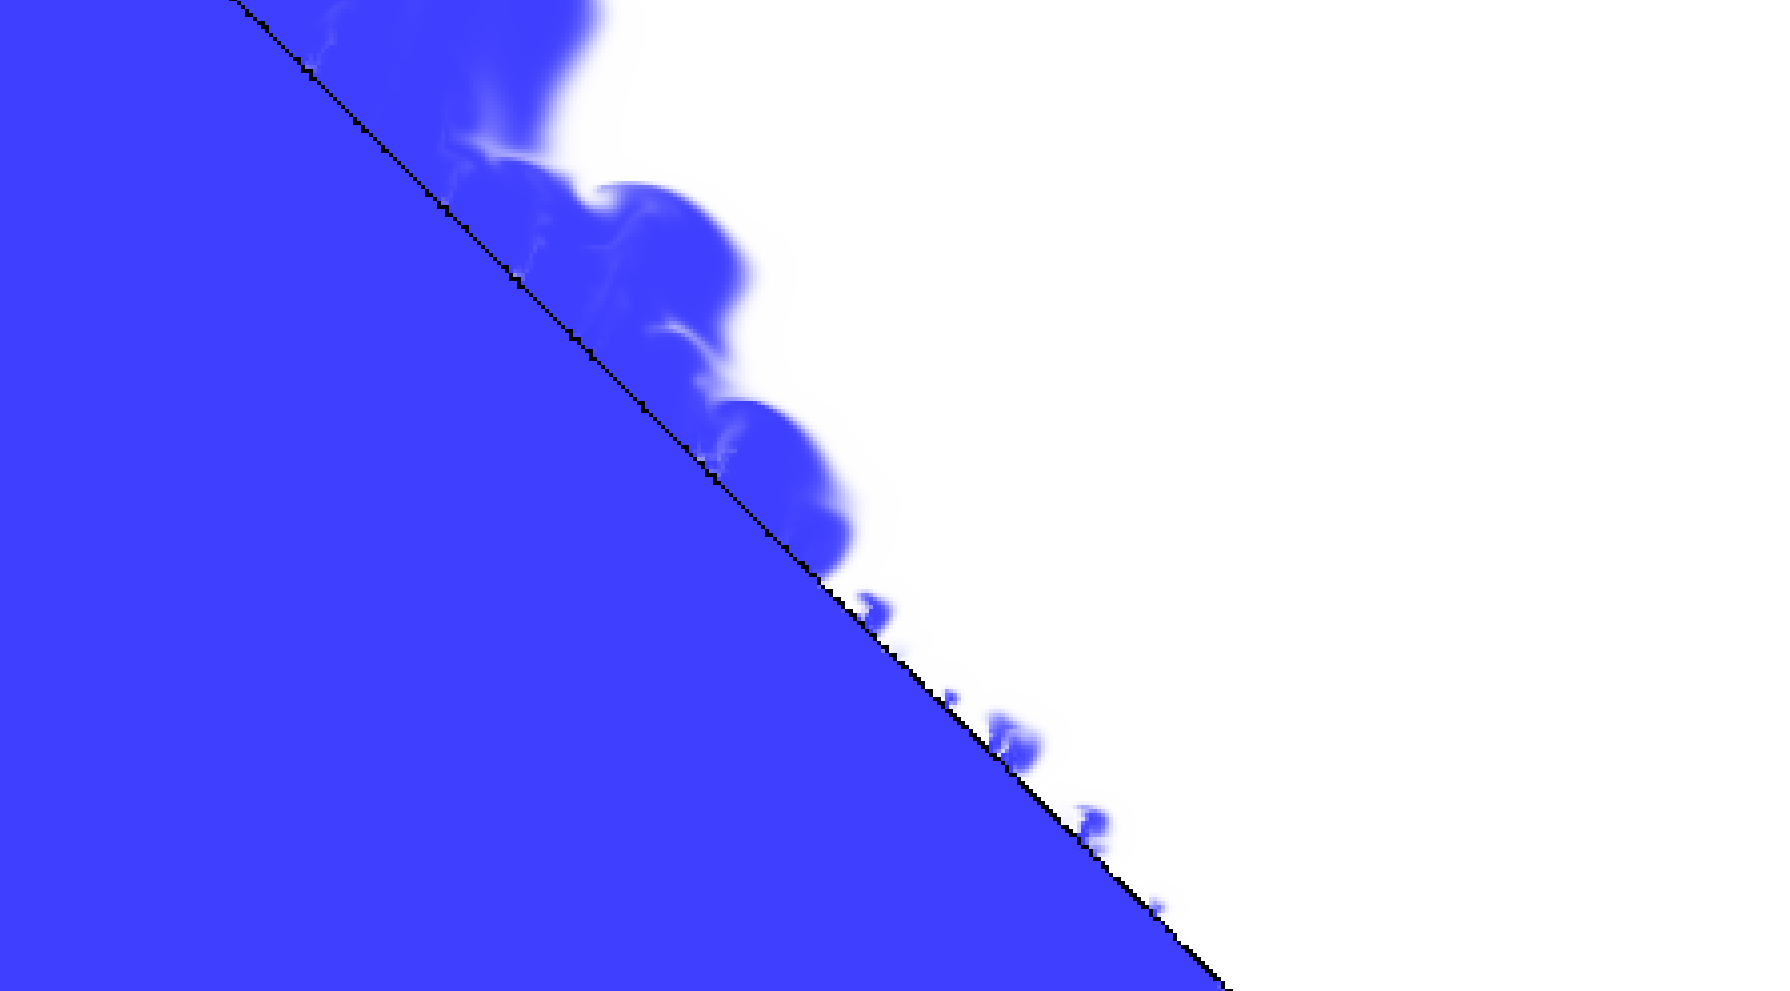
\includegraphics[width=0.9\textwidth]{fuites.png}}
    \end{column}

    % --- Séparateur vertical ---
    \begin{column}{0.04\textwidth}
        
        \begin{tikzpicture}[baseline=(current bounding box.center)]
            \draw[very thick,gray!60] (0,0) -- (0,4.5);
        \end{tikzpicture}
    \end{column}

    % --- Colonne de droite ---
    \begin{column}{0.48\textwidth}
        \centering
        \boxed{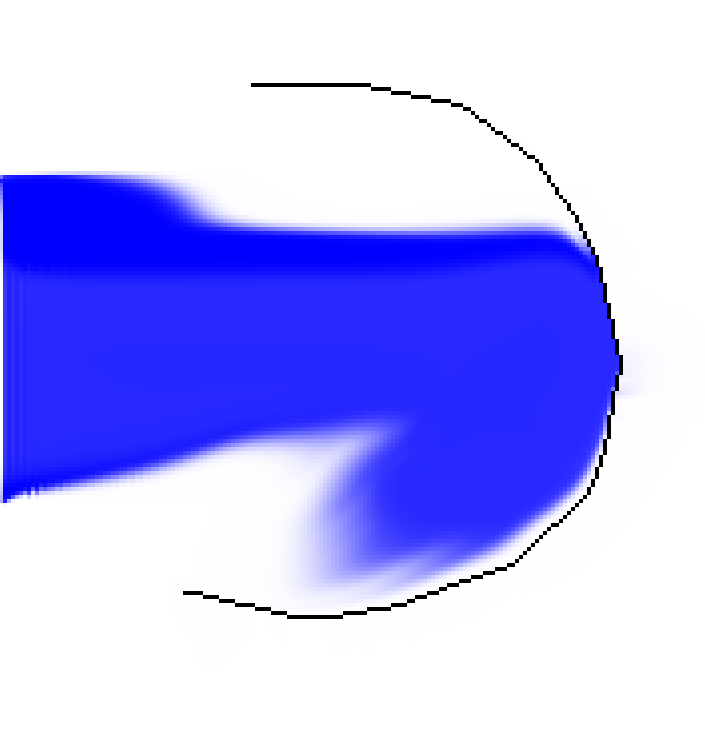
\includegraphics[width=0.8\textwidth]{pertes.png}}
    \end{column}
   
\end{columns}
\vspace{6mm}
· Nouveau solveur : CIP-CSL4 infructueux
\end{frame}

\begin{frame}{}
    \textbf{Potentielles améliorations:}
    \begin{itemize}
        \item · Régler les problèmes de conservation de la masse du fluide
        \item · Passer à une grille de taille adaptative 
        \item · Passer à un univers en 3D et infini
        \item · Mise en place d'un système de cassure des solides
    \end{itemize}

    \vspace{0.5cm}

    \begin{columns}
        \begin{column}{0.48\textwidth}
            \centering
            \boxed{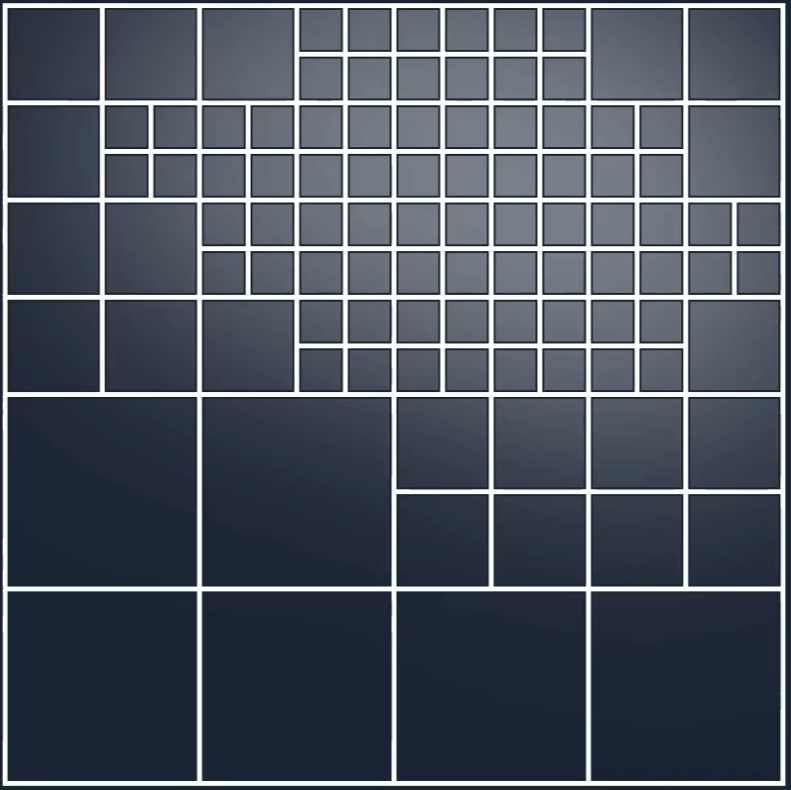
\includegraphics[width=0.6\textwidth]{./Amelioration_adaptative_grid.png}}
        \end{column}
        \begin{column}{0.04\textwidth}
            
            \begin{tikzpicture}[baseline=(current bounding box.center)]
                \draw[very thick,gray!60] (0,0) -- (0,3.5);
            \end{tikzpicture}
        \end{column}
        \begin{column}{0.48\textwidth}
            \centering
            \boxed{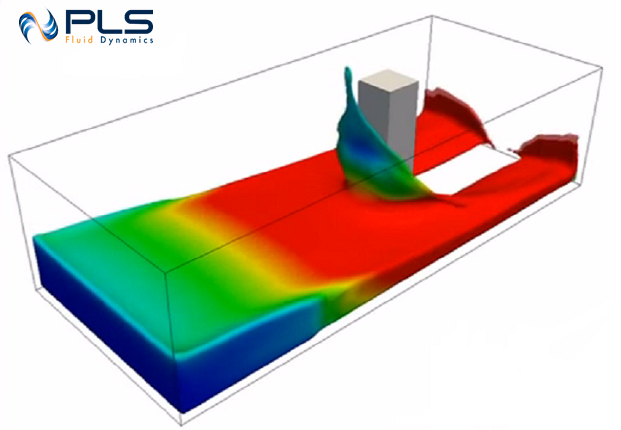
\includegraphics[width=0.8\textwidth]{./sim3D.png}}
        \end{column}
    \end{columns}
    

\end{frame}


\end{document}